%!TEX program = xelatex
%!BIB program = biber
\documentclass[cn, 12pt, math=mtpro2, bibstyle=apa, blue, twocol]{elegantbook}
\title{高级微观经济学}
\subtitle{Advanced Microeconomics}

\setcounter{tocdepth}{3}
\cover{cover.png}

\date{\today}

\addbibresource[location=local]{reference.bib}

\usepackage{cprotect}
\usepackage{array}
\usepackage{bbm}
\usepackage{pgfplots}
\pgfplotsset{compat = newest}
\usetikzlibrary{positioning, arrows.meta}
\usepgfplotslibrary{fillbetween}
\newcommand{\ccr}[1]{\makecell{{\color{#1}\rule{1cm}{1cm}}}}

\definecolor{customcolor}{RGB}{249,203,142}
\colorlet{coverlinecolor}{customcolor}

\newcommand*{\rom}[1]{\expandafter\@slowromancap\romannumeral #1@}
\newcommand{\R}{\mathbb{R}}
\newcommand{\p}{\mathbf{p}}
\newcommand{\x}{\mathbf{x}}
\newcommand{\overbar}[1]{\mkern 1.5mu\overline{\mkern-1.5mu#1\mkern-1.5mu}\mkern 1.5mu}

\emergencystretch=4em
\begin{document}

\maketitle
\frontmatter

\tableofcontents

\mainmatter
\chapter{消费者理论\rom{1}}
\section{基本概念}
\textbf{消费集} (consumption set)消费者能想到的所有选择或者全部消费方案的集合, 不管其中的某些选择在现实中能否实现. 消费集也称选择集 (choice set), 用大写字母$X$表示.

假设每种商品是无限细分的, $x_i\in\R_+$表示商品$i$的数量, 这里假设每种商品数量非负且允许某些商品数量为0. 进一步, 假设有$n$种商品, 并用
$$\x=\begin{pmatrix}
      x_1 \\
      \vdots \\
      x_n
    \end{pmatrix}\in \R^n_+$$
表示含有$n$种商品的\textbf{消费束} (consumption bundle)或\textbf{消费计划} (consumption plan), $\R^n_+$称为商品空间 (commodity space). 因此, 消费束$\x\in X$可用$\R^n_+$中的点表示, 出于简单起见, 这里用整个$\R^n_+$表示消费集$X$.

\begin{postulate}\label{pos:pos1.1}
消费集的最低要求: 1. $X\subset \R_+^n$; 2. $X$是闭集和凸集; 3. $\mathbf{0}\in X$.
\end{postulate}

\textbf{可行集} (feasible set)是消费者脑海里能想到的, 并且在所处环境中所能得到的消费集, 用大写字母$B$表示, 它是$X$的真子集.

\textbf{偏好关系} (preference relation)为消费者的购买欲望, 反映消费者的主观愿望, 其为理想竞争市场的一个限制因素.
\section{偏好与效用}
\subsection{偏好关系}
消费者在$X$中的偏好关系$\succsim$可用来表示他对不同消费束的偏好, 如果$\x^1\succsim\x^2$, 那么对这个消费者来说, 称“$\x^1$至少和$\x^2$一样好”. 在消费者选择公理下, 消费者能够进行选择而且这些选择以某特定方式保持一致性.

进一步, 我们可以从偏好关系$\succsim$推导出$X$上的另外两种关系
\begin{itemize}
  \item 严格偏好关系 (strictly preference relation): $\x^1\succ \x^2 \Leftrightarrow \x^1\succsim \x^2$且$ \x^1\succsim \x^1$不成立, 称“$\x^1$严格好于$\x^2$”.
  \item 无差异关系 (indifference relation): $\x^1\sim \x^2 \Leftrightarrow \x^1\succsim \x^2$且$\x^2\succsim \x^1$, 称“$\x^1$和$\x^2$一样好”.
\end{itemize}
在大部分经济理论中, 经济学家都假设个人偏好是理性的 (rational), 这个假设体现在关于偏好关系$\succsim$的两个基本公理上, 即完备性公理和传递性公理.

\begin{axiom}[完备性]\label{axi:axi1.1}
对于任意$\x^1, \x^2\in X$, 要么$\x^1\succsim \x^2$, 要么$\x^2\succsim \x^1$.
\end{axiom}
完备性表明, 消费者具有分辨消费集内任意消费束的能力, 可以比较出是$\x^1$至少和$\x^2$一样好, 还是$\x^2$至少和$\x^1$一样好. 通常而言, 这条公理在现实中通常都是成立的.

\begin{axiom}[传递性]\label{axi:axi1.2}
对于$X$中的任意消费束$\x^1$, $\x^2$和$\x^3$, 如果$\x^1\succsim \x^2$且$\x^2\succsim\x^3$, 那么$\x^1\succsim\x^3$.
\end{axiom}
传递性要求消费者的选择必须一致. 然而, 这一公理是备受争议的, 人类的选择不总是传递的, 如果决策者评估的备选物不在他的常识范畴之内, 那么传递性这个公理很难得到满足, 但尽管如此还是认为传递性公理总是成立.

若把这两条公理结合起来, 这就意味着消费者能够将消费集$X$中的任何有限个元素全部排列起来, 排列顺序为从最好到最差, 当然可能会出现某些元素一样好的局面.
\begin{definition}[理性偏好关系]
如果消费集$X$上的偏好关系$\succsim$满足公理\ref{axi:axi1.1}和\ref{axi:axi1.2}, 则称$\succsim$为一个理性偏好关系.
\end{definition}
理性偏好关系$\succsim$是完备的和传递的, 蕴含着严格偏好$\succ$和无差异$\sim$的性质, 我们将这些性质总结在命题\ref{pro:pro1.1}中.
\begin{proposition}\label{pro:pro1.1}
  如果偏好关系$\succsim$是理性的, 那么下列结论成立
  \begin{enumerate}[\arabic*.]
    \item 如果$\x^1\succ\x^2\succsim\x^3$, 那么$\x^1\succ\x^3$;
    \item 如果$\x^1\succ\x^2$且$\x^2\succ\x^3$, 那么$\x^1\succ\x^3$;
    \item 如果$\x^1\sim\x^2$且$\x^2\sim\x^3$, 那么$\x^1\sim\x^3$并且$\x^2\sim \x^1$.
  \end{enumerate}
\end{proposition}
\begin{proof}
  1. 由于$\x^1\succ\x^2$意味着$\x^1\succsim \x^2$, 传递性表明$\x^1\succsim \x^3$. 假设$\x^3\succsim\x^1$, 由于$\x^2\succsim \x^3$, 因此传递性意味着$\x^2\succsim \x^1$, 但这与$\x^1\succ \x^2$矛盾, 故而只有$\x^1\succ\x^3$.

  2. 原理同上.

  3. 假设$\x^1\sim\x^2$且$\x^2\sim\x^3$, 那么$\x^1\succsim\x^2$, $\x^2\succsim\x^3$, $\x^2\succsim\x^1$, $\x^3\succsim\x^2$, 传递性意味着$\x^1\succsim\x^3$且$\x^3\succsim\x^1$, 也即$\x^1\sim\x^3$. 另一方面, $\x^1\sim \x^2$意味着$\x^2\succsim\x^1$且$\x^1\succsim\x^2$, 也即$\x^2\sim\x^1$.
\end{proof}
\begin{definition}
设$\x^0$是消费集$X$内的任意一点, 与$\x^0$相联系, 可以定义$X$的子集
\begin{enumerate}[label=\arabic*.]
  \item $\succsim(\x^0)\equiv \{\x: \x\in X, \x\succsim\x^0\}$, 称为“至少和$\x^0$一样好”的集合;
  \item $\precsim(\x^0)\equiv \{\x: \x\in X, \x^0\succsim\x\}$, 称为“不比$\x^0$好”的集合;
  \item $\succ(\x^0)\equiv \{\x: \x\in X, \x\succ\x^0\}$, 称为“比$\x^0$好”的集合;
  \item $\prec(\x^0)\equiv \{\x: \x\in X, \x^0\succ \x\}$, 称为“比$\x^0$差”的集合;
  \item $\sim(\x^0)\equiv\{\x: \x\in X, \x\sim \x^0\}$, 称为“与$\x^0$无差异”的集合.
\end{enumerate}
\end{definition}

对于消费集$X=\R_+^2$, 图\ref{fig1.1}表示了一个理性的虚拟偏好集, $X$中的任意一点$\x^0=(x_1^0,x_2^0)'$表示该消费束中商品1和2的数量分别为$x_1^0$和$x_2^0$, 并且集合$\succ(\x^0)$, $\prec(\x^0)$和$\sim(\x^0)$将整个$X$划分为了三个互不相交的子集.
\begin{figure}
  \centering
  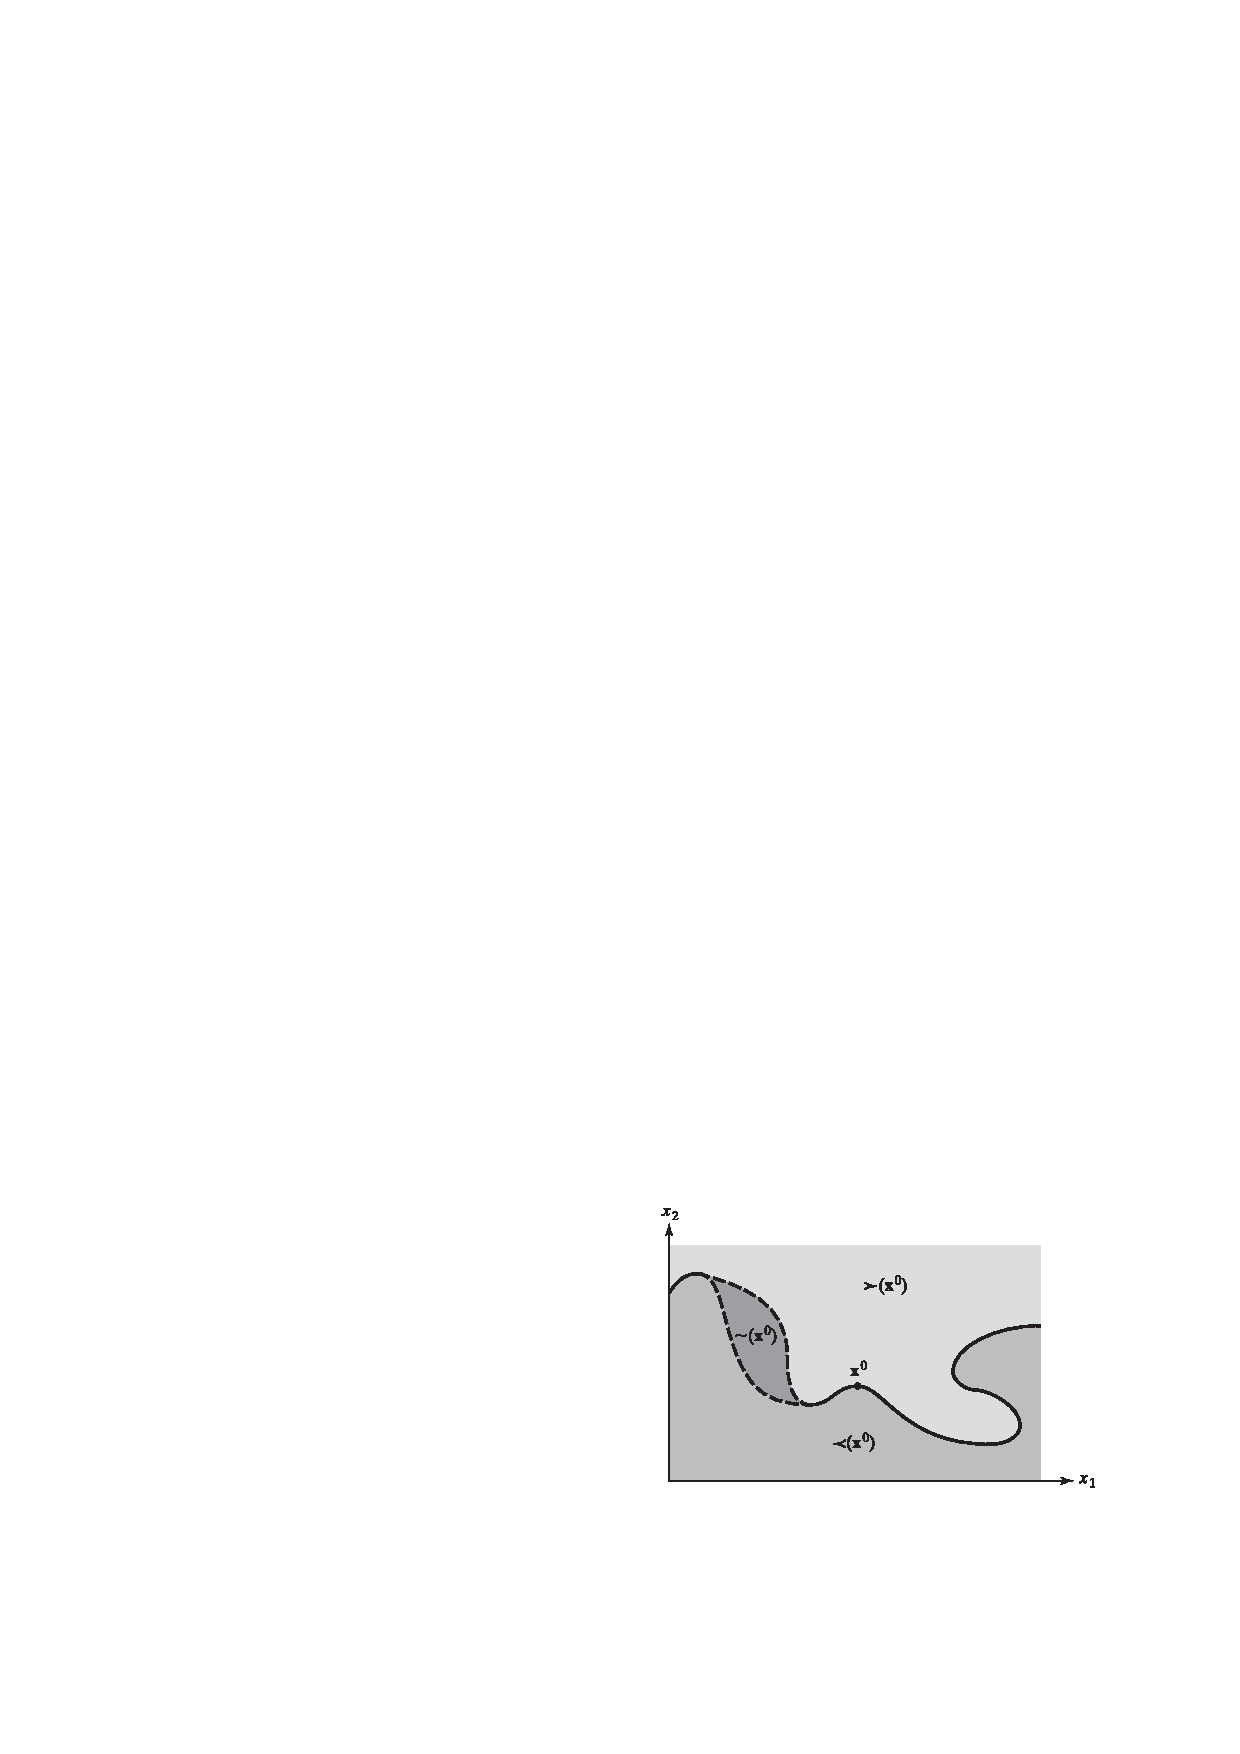
\includegraphics[width=10cm]{fig1.pdf}
  \caption{理性虚拟偏好.}\label{fig1.1}
\end{figure}

由于还未给出其它公理, 理性偏好允许了图\ref{fig1.1}中不规则区域的存在, 例如无差异区域内部的空隙. 以下明确地将消费集设置为$X=\R^n_+$.

\begin{axiom}[连续性]\label{axi:axi1.3}
对于任意$\x\in\R^n_+$, 集合$\succsim(\x)$和$\precsim(\x)$在$\R_+^n$中是闭的.
\end{axiom}
连续性公理保证了偏好不会发生突然逆转. 如果消费束序列中的每个元素$\mathbf{y}^n$至少与$\x$一样好, 并且$\mathbf{y}^n$收敛于$\mathbf{y}$, 则$\mathbf{y}$至少与$\x$一样好. 由于$\succsim(\x)$和$\precsim(\x)$是闭的, 因此它们的交集$\sim(\x)$也是闭的, 这就排除了图\ref{fig1.1}中虚线的存在, 图\ref{fig1.2}画出了满足连续性的理性虚拟偏好.

\begin{figure}[htbp!]
  \centering
  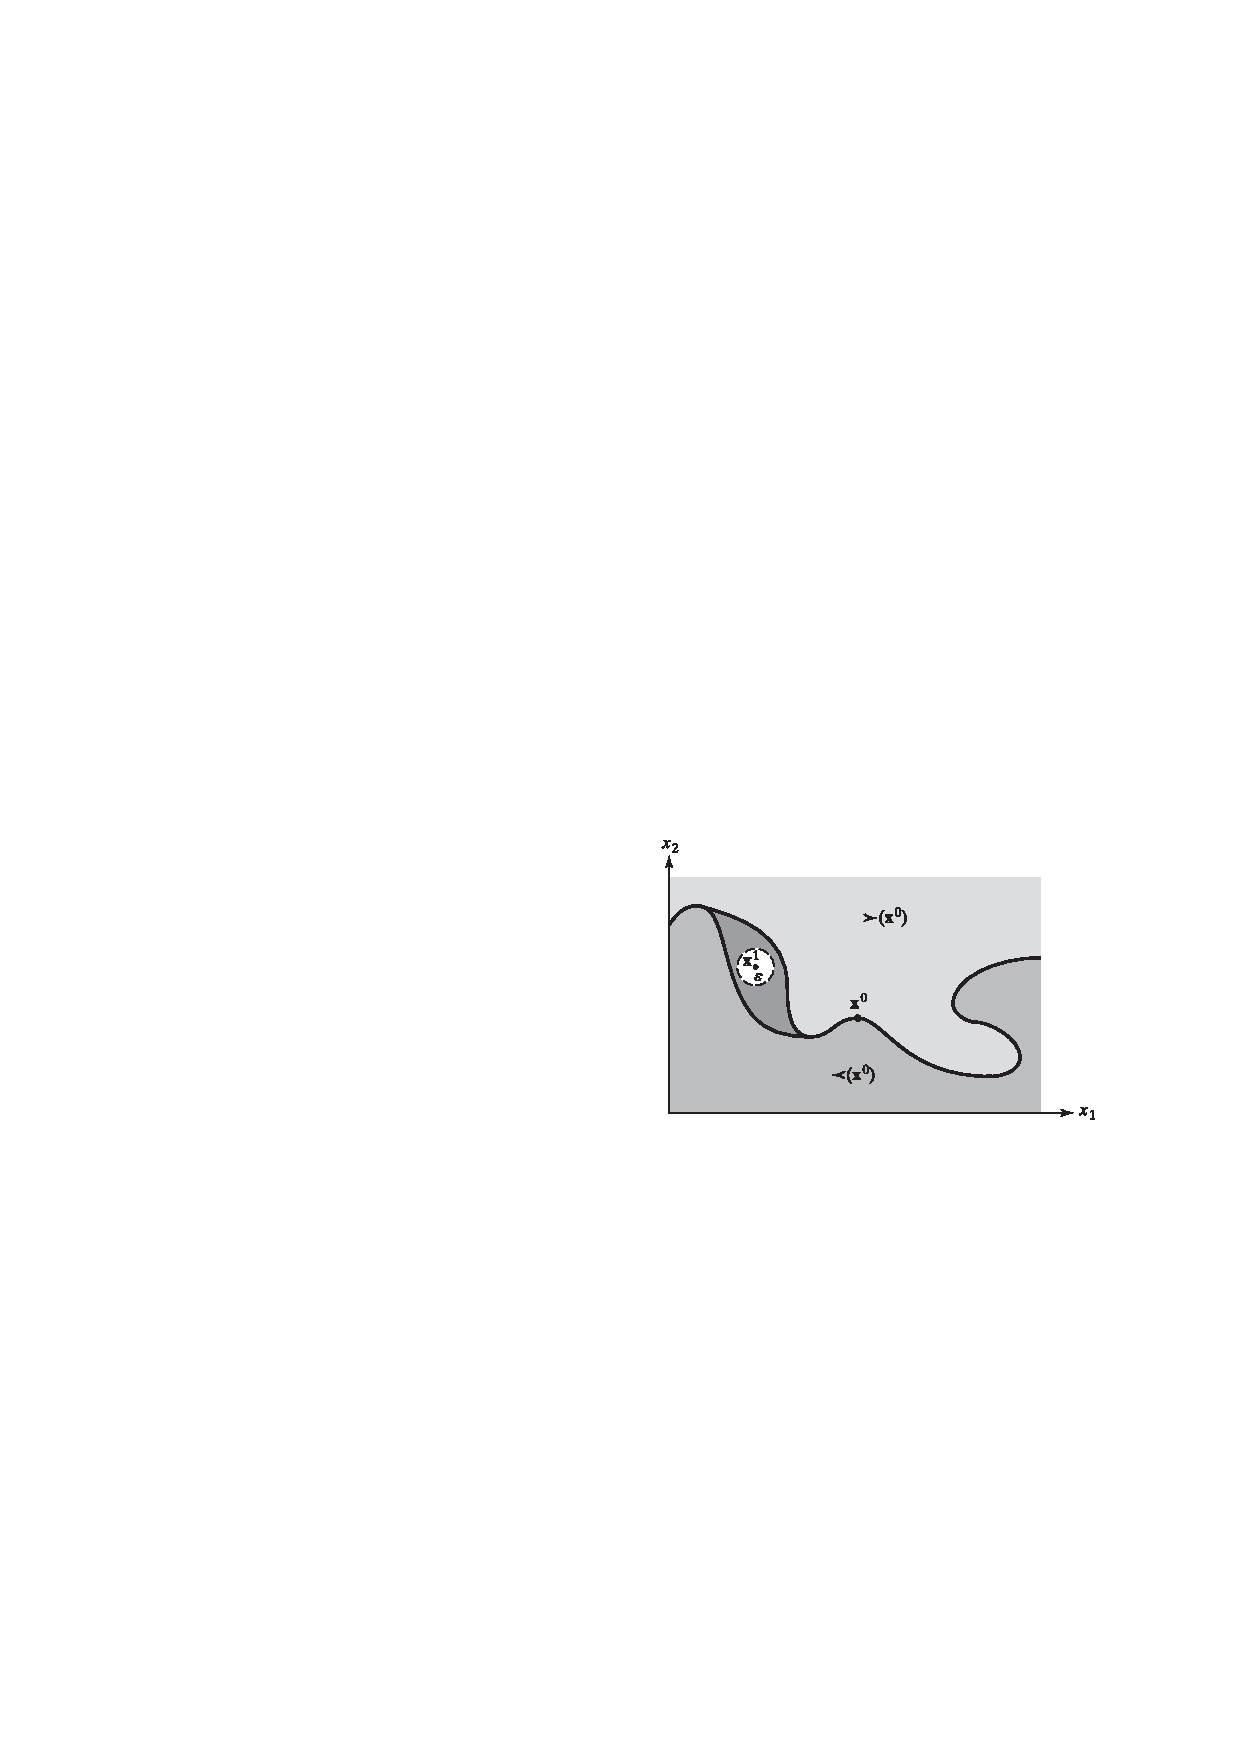
\includegraphics[width=10cm]{fig2.pdf}
  \caption{满足公理\ref{axi:axi1.3}的理性虚拟偏好.}\label{fig1.2}
\end{figure}

\begin{example}[字典偏好关系]
假设$X=\R_+^2$, 将偏好关系$\succsim$定义为要么$x_1>y_1$, 要么$x_1=y_1$且$x_2\ge y_2$, 则称$\succsim$是字典偏好关系. 可以证明, 字典偏好关系不是连续的.
\end{example}

接下来的几条假设将使的偏好的结构更复杂但更规则, 如果说前面的三条公理是必须的, 那么下面的这类假设则要根据具 体研究的选择决策问题来决定是否使用. 在下面每类假设中, 先介绍较弱的公理, 然后再介绍较强的公理.

\begin{axiom}[局部非饱和性]\label{axi:axi1.4}
对于任意$\x^0\in\R^n_+$以及$\epsilon>0$, 总存在$\x\in B_\varepsilon(\x^0)\cap \R_+^n$, 使得$\x\succ\x^0$.
\end{axiom}
局部非饱和性排除了无差异区域的存在, 因为在无差异区域中, 总能找到某个$\epsilon>0$和$B_\epsilon(\x^1)$, 使得$B_\epsilon(\x^1)$中的点和$\x^1$无差异, 如图\ref{fig1.3}所示.
\begin{figure}
  \centering
  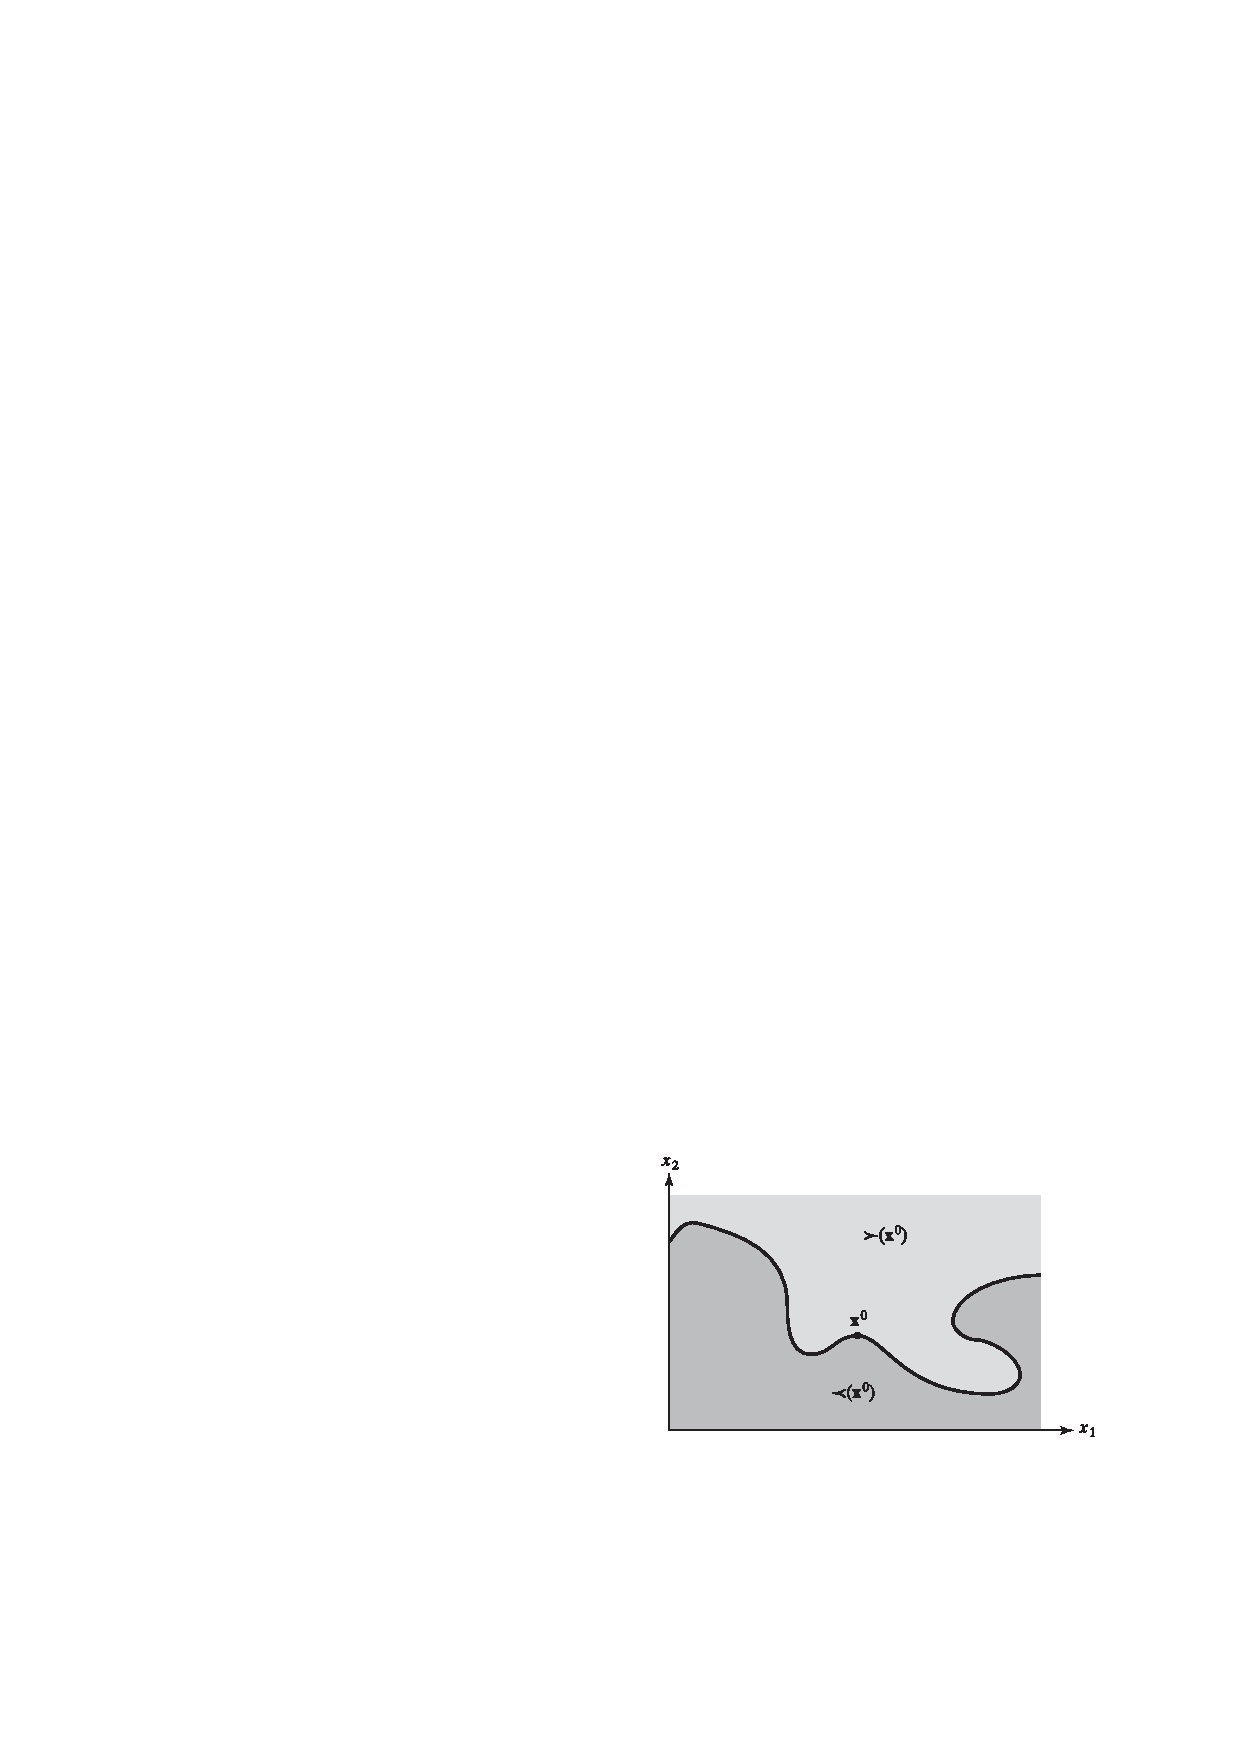
\includegraphics[width=10cm]{fig3.pdf}
  \caption{满足公理\ref{axi:axi1.3}和\ref{axi:axi1.4}的理性虚拟偏好.}\label{fig1.3}
\end{figure}

然而, 这并不意味着增加所有商品的数量必然能使消费者的状况更好, 以下更强的严格单调性公理则表明了这一点.

\begin{axiom}[严格单调性]\label{axi:axi1.5}
对于任意$\x^0,\x^1\in\R^n_+$, 如果$\x^0\ge\x^1$, 那么$\x^0\succsim \x^1$; 如果$\x^0>>\x^1$, 那么$\x^0\succ\x^1$.
\end{axiom}
严格单调性表明如果某消费束的每种商品数量至少和另一个消费束的一样多, 则该消费束至少和它一样好; 如果某消费束的每种商品严格多于另一个消费束, 则该消费束比后者好. 此外, 这一公理排除了$\R^2_+$中无差异集中的向上弯曲部分和斜率为正的部分, 如图\ref{fig1.4}所示.

\begin{figure}
  \centering
  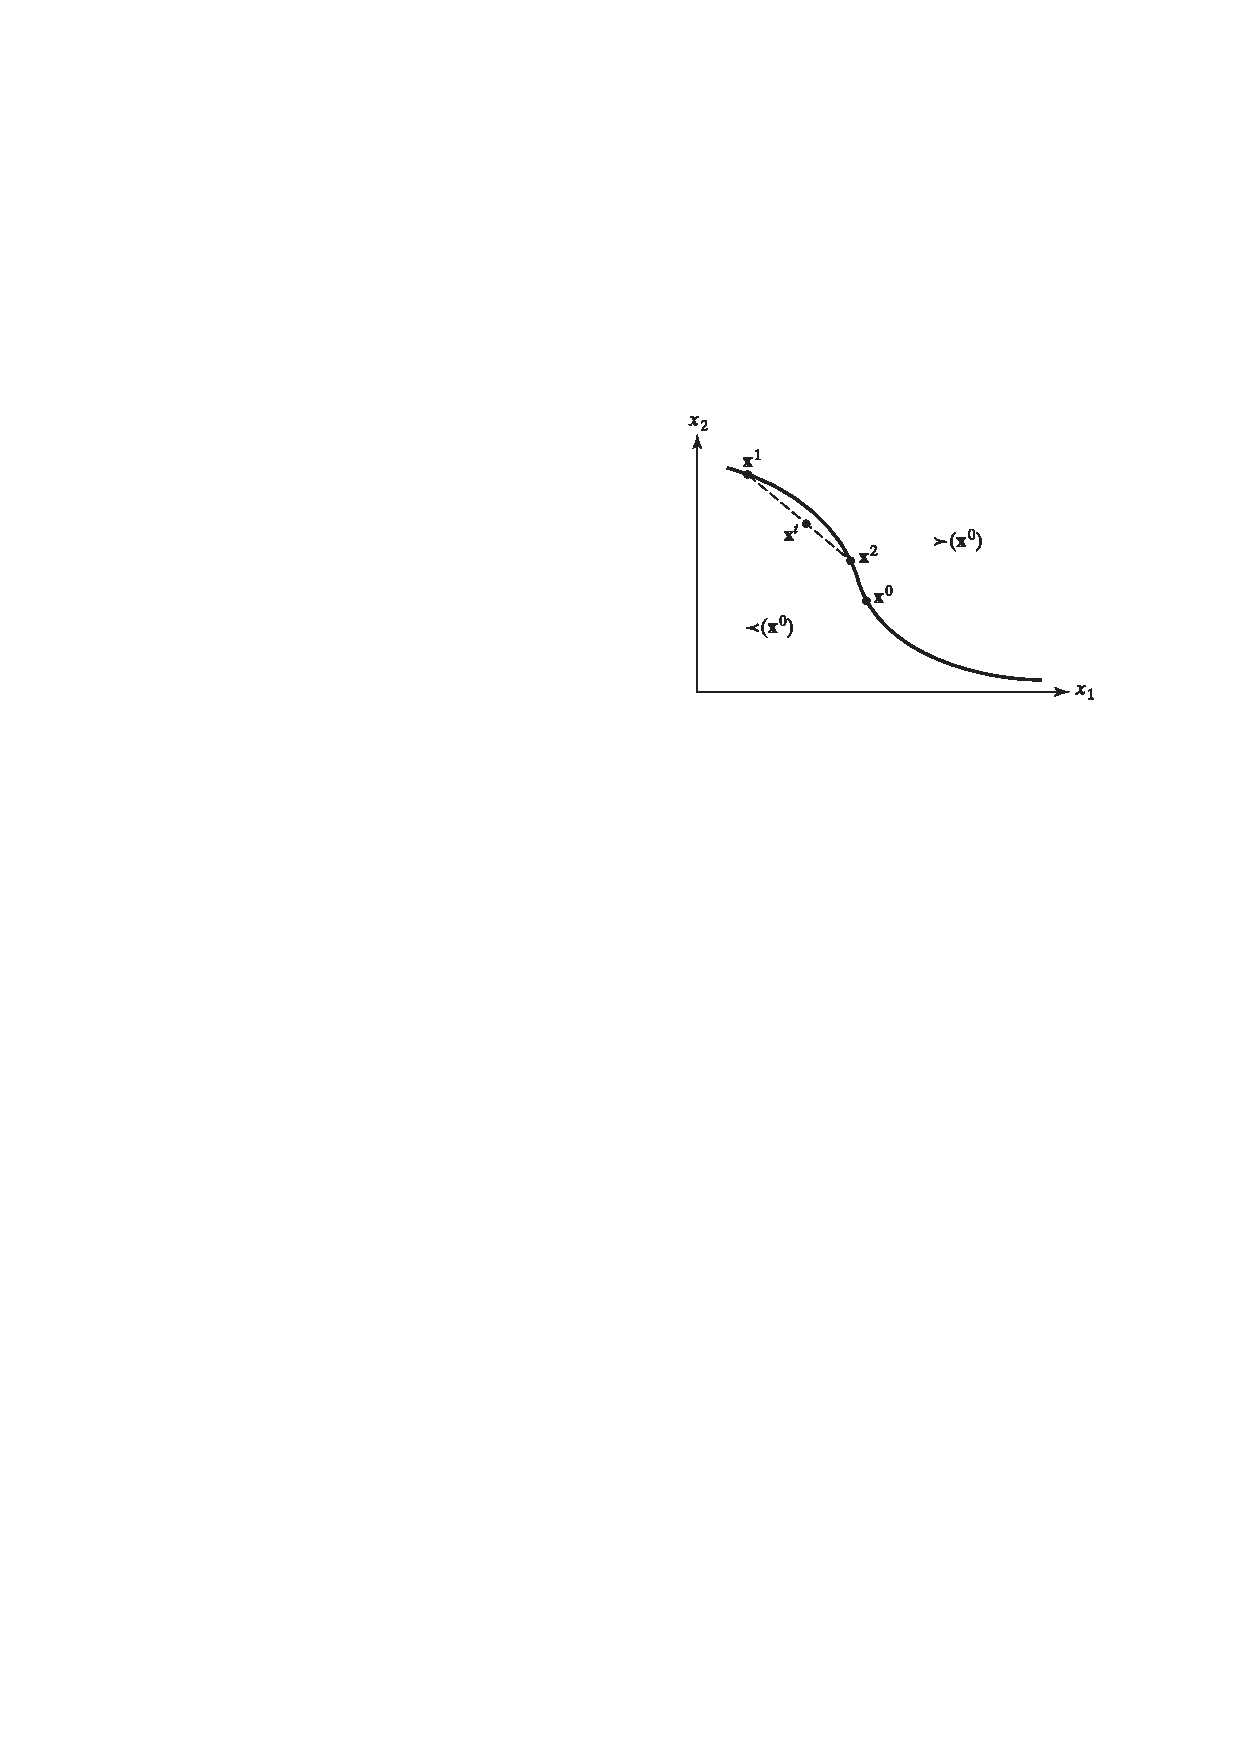
\includegraphics[width=10cm]{fig4.pdf}
  \caption{满足公理\ref{axi:axi1.3}和\ref{axi:axi1.5}的理性虚拟偏好.}\label{fig1.4}
\end{figure}

\begin{axiom}[凸性]\label{axi:axi1.6}
如果$\x^1\succsim\x^0$, 则对于一切$t\in[0,1]$都有$t\x^1+(1-t)\x^0\succsim\x^0$.
\end{axiom}
\begin{axiom}[严格凸性]\label{axi:axi1.7}
如果$\x^1\ne\x^0$且$\x^1\succsim\x^0$, 则对于一切$t\in(0,1)$都有$t\x^1+(1-t)\x^0\succ\x^0$.
\end{axiom}

如果凸性或严格凸性与公理\ref{axi:axi1.1}、\ref{axi:axi1.2}、\ref{axi:axi1.3}和\ref{axi:axi1.5}联合起来, 那么可以排除图\ref{fig1.4}中西北方向凹向原点的部分, 如图\ref{fig1.5}所示.

对于我们将要构造的消费者理论来说, 引入公理\ref{axi:axi1.6}不会造成理论一般性的任何损失. 引入或不引入这个公理, 消费者理论的内容是相同的. 若引入公理\ref{axi:axi1.7}, 则多少会造成一般性的损失, 但是它可以大幅简化我们的分析.

描述凸偏好的另一种方式是\textbf{曲率} (curvature), 当消费集为$X=\R^2_+$, 无差异曲线的斜率称为商品1对商品2的\textbf{边际替代率} (Marginal Rate of Substitution, MRS), 它衡量为了维持相同的效用水平, 消费者减少1单位商品1的消费, 应该补偿给她多少商品2.

当公理\ref{axi:axi1.6}成立时, 如果沿着无差异曲线从西北到东南移动, 那么MRS不变或递减, 而如果公理\ref{axi:axi1.7}成立, 则要求MRS严格递减. 凸偏好的这种性质称为边际替代率递减规律.
\begin{figure}
  \centering
  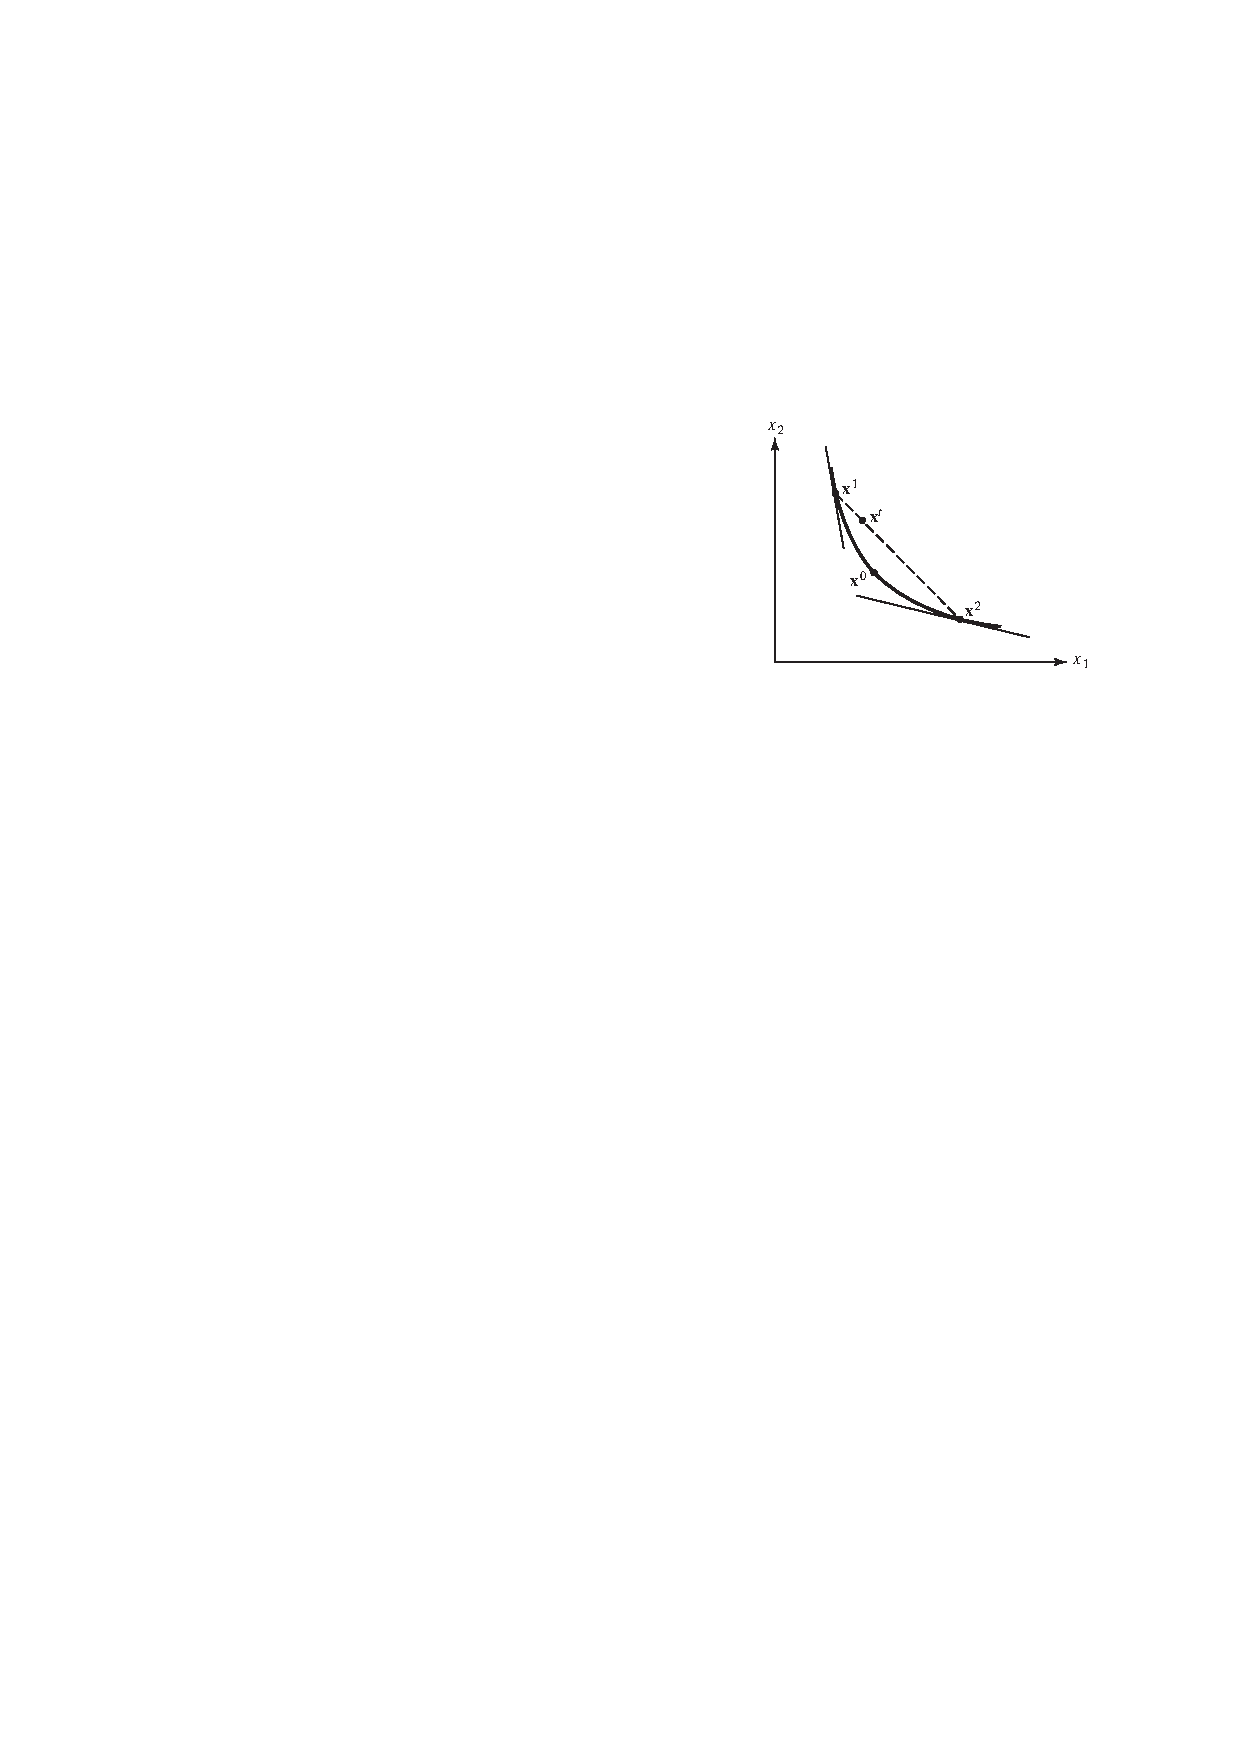
\includegraphics[width=10cm]{fig5.pdf}
  \caption{满足公理\ref{axi:axi1.3}、\ref{axi:axi1.5}、\ref{axi:axi1.6}或\ref{axi:axi1.7}的理性虚拟偏好.}\label{fig1.5}
\end{figure}
\subsection{效用函数}
\begin{definition}
实值函数$u:\R_+^n\to\R$称为表示偏好关系$\succsim$的效用函数 (utility function), 如果对于一切$\x^0, \x^1\in\R^n_+$, 都有$u(\x^0)\ge u(\x^1)\Leftrightarrow \x^0\succsim\x^1$.
\end{definition}
表示偏好关系$\succsim$的效用函数不是唯一的, 对于任意严格递增的单调函数$f:\R\to\R$来说, $v(\x)=f(u(\x))$都是一个新的效用函数, 它与$u(\x)$表示的偏好相同. 效用函数这种不随任何严格递增变换而改变的性质称为\textbf{序数} (ordinal)性质, 而\textbf{基数} (cardinal)性质则是指在这样的变换下不能保留的性质.

\begin{proposition}
只有理性偏好才能用效用函数表示.
\end{proposition}
\begin{proof}
 只需证明若存在能表示偏好关系$\succsim$的效用函数, 则$\succsim$必然满足公理\ref{axi:axi1.1}和\ref{axi:axi1.2}.

 因为$u$是定义在$\R_+^n$上的实值函数, 那么对于任意$\x,\mathbf{y}\in\R_+^n$, 必有$u(\x)\ge u(\mathbf{y})$或$u(\x)\le u(\mathbf{y})$, 由于$u$是表示偏好关系$\succsim$的效用函数, 因此$\x\succsim \mathbf{y}$和$\mathbf{y}\succsim\x$总有一个成立, 也即偏好关系$\succsim$满足公理\ref{axi:axi1.1}.

 假设对于任意$\x, \mathbf{y}, \mathbf{z}\in\R_+^n$都有$\x\succsim\mathbf{y}$且$\mathbf{y}\succsim\mathbf{z}$, 那么$u(\x)\ge u(\mathbf{y})$且$u(\mathbf{y})\ge u(\mathbf{z})$, 也即$u(\x)\ge u(\mathbf{z})$, 因为$u$表示了偏好关系$\succsim$, 故而$\x\succsim\mathbf{z}$, 也即公理\ref{axi:axi1.2}成立.
\end{proof}

\begin{theorem}\label{thm:thm1.1}
  如果理性偏好$\succsim$是连续和严格单调的, 那么存在可以代表$\succsim$的连续效用函数$u:\R^n_+\to\R$.
\end{theorem}
\begin{proof}
  令$\mathbf{e}=(1,\cdots,1)'\in\R^n_+$为单位向量, 首先证明存在映射$u:\R^n_+\to\R$, 使得$u(\x)\mathbf{e}\sim \x$.

  固定消费束$\x\in\R^n_+$, 根据连续性公理可知集合
  \begin{align*}
  A^+&=\{t\ge0: t\mathbf{e}\succsim \x\} \\
  A^-&=\{t\ge0: t\mathbf{e}\precsim \x\}
  \end{align*}
  都是非空闭集. 由于偏好关系$\succsim$是完备的, 故而$\R_+\subset A^+\cup A^-$, 又因为$A^+$和$A^-$是闭的, 并且$\R_+$是连通的, 所以$A^+\cap A^-\neq\emptyset$, 于是存在$t\ge0$使得$t\mathbf{e}\sim \x$. 假设还存在另一个$t'\ge0$使得$t'\mathbf{e}\sim \x$, 根据命题\ref{pro:pro1.1}可知$t\mathbf{e}\sim t'\mathbf{e}$, 于是由严格单调性知$t=t'$, 也即这样的$t$是唯一的.

  由上面的论证可知, 对于任意$\x\in\mathbb{R}_+^n$, 总存在唯一的实数$u(\x)$使得$u(\x)\mathbf{e}\sim\x$, 下面证明$u$代表了偏好关系$\succsim$. 给定消费束$\x^1, \x^2\in\R_+^n$, 于是
  \begin{align*}
  \x^1\succsim\x^2&\Leftrightarrow u(\x^1)\mathbf{e}\sim \x^1\succsim u(\x^2)\mathbf{e}\sim \x^2 \\
  &\Leftrightarrow u(\x^1)\mathbf{e}\succsim u(\x^2)\mathbf{e} \\
  &\Leftrightarrow u(\x^1)\ge u(\x^2)
  \end{align*}
  这就得到了可以表示偏好关系$\succsim$的效用函数的存在性.

  最后需要证明效用函数$u:\R^n_+\to \R$是连续的, 注意到对于每个$a<b$都有
  \begin{align*}
  u^{-1}((a,b))&=\{\x: a<u(\x)<b\} \\
  &=\{\x: a\mathbf{e}\prec u(\x)\mathbf{e}\prec b\mathbf{e}\} \\
  &=\{\x: a\mathbf{e}\prec \x\mathbf{e}\prec b\mathbf{e}\} \\
  &=\succ (a\mathbf{e})\,\,\cap \prec(b\mathbf{e})
  \end{align*}
  根据连续性可知$\succ(a\mathbf{e})$和$\prec(b\mathbf{e})$是开的, 由于开集的交也是开的, 因此$u^{-1}((a,b))$是开的, 故而由连续函数的定义可知$u$是连续的.
\end{proof}

连续的理性偏好排除了病态的效用函数, 但是它没有排除出现拐折 (kink)函数情形, 例如Leontief偏好, 而如果效用函数是可微的, 那么无差异曲线不仅是连续曲线, 并且还是光滑的. 因此, 效用函数的可微性比连续性要求更高, 可微效用函数也不一定能表示某些连续偏好, 但通常在需要的时候就假设$u$是可微的.


当效用函数可微时, $u(\x)$对$x_i$的一阶偏导为商品$i$的\textbf{边际效用} (marginal utility), 考虑任意消费束$\x^1=(x^1_1,x^2_2)$, 因为经过点$\x^1$的无差异曲线是平面$(x_1,x_2)$的函数, 令$x_2=f(x_1)$为这一函数, 因此当效用水平维持在常数时, 对于一切$\x\in\R_+$都有
\begin{equation}\label{eq1.1}
  u(x_1,f(x_1))=\text{常数}
\end{equation}
对于消费束$\x^1=(x^1_1,x^1_2)$, 商品1替代商品2的边际替代率$\text{MRS}_{12}$为经过点$(x_1^1,x_2^1)$的无差异曲线在该点的斜率的绝对值, 也即
$$\text{MRS}_{12}(x_1^1,x_2^1)=|f'(x_1^1)|=-f'(x_1^1)$$
在式(\ref{eq1.1})中对$x_1$求微分
\begin{equation}\label{eq1.2}
  \frac{\partial u}{\partial x_1}+\frac{\partial u}{\partial x_2}f'(x_1)=0
\end{equation}
根据式(\ref{eq1.1})和(\ref{eq1.2})可得
$$\text{MRS}_{12}(\x^1)=\frac{\partial u(\x^1)/\partial x_2}{\partial u(\x^1)/\partial x_1}$$
一般地, 对于某个消费者来说, 商品$i$对商品$j$的边际替代率为
$$\text{MRS}_{ij}(\x)=\frac{\partial u(\x)/\partial x_j}{\partial u(\x)/\partial x_i},\quad i,j=1,\cdots,n$$
当$u(\x)$在$\R^n_{++}$上可微并且它表示的偏好关系$\succsim$严格单调时, 每种商品的边际效用“几乎”严格为正,\footnote{“几乎”表示除开Lebesgue测度为0的消费束$\x$.} 也即几乎对于一切消费束$\x$都有$\partial u(\x)/\partial x_j>0$. 更一般地, 对于任何拟凹效用函数, 由它的二阶偏导构成的Hessian矩阵$\mathbf{H}(\x)$满足
$$\mathbf{y}'\mathbf{H}(\x)\mathbf{y}\le0,\quad \nabla u(\x)\cdot\mathbf{y}=0$$

  \begin{theorem}\label{thm:thm1.2}
    设偏好关系$\succsim$可由效用函数$u:\R_+^n\to\R$表示, 则以下结论成立:
    \begin{enumerate}[label=\arabic*.]
      \item $u$是严格递增函数当且仅当$\succsim$是严格单调的;
      \item $u$是拟凹函数当且仅当$\succsim$是凸的;
      \item $u$是严格拟凹函数当且仅当$\succsim$是严格凸的.
    \end{enumerate}
  \end{theorem}
  \begin{proof}
    1. 设$\x\ge \mathbf{y}$且$u$是严格递增的, 于是$u(\x)\geq (\mathbf{y})\Leftrightarrow \x\succsim \mathbf{y}$; 反之, 如果$\succsim$是严格单调的, 那么当$\x\ge\mathbf{y}$是有$\x\succsim\mathbf{y}$, 从而$u(\x)\ge u(\mathbf{y})$, 也即$u$是严格递增的.

    2. 设$u$是拟凹函数, 也即对于任意$t\in [0,1]$都有$u(t\x+(1-t)\mathbf{y})\geq \min\{u(\x), u(\mathbf{y})\}$. 不妨设$\x\succsim \mathbf{y}$, 从而$t\x+(1-t)\mathbf{y}\succsim \mathbf{y}$, 也即$\succsim$是凸的; 反之, 假设$\succsim$是凸的并且$\x\succsim\mathbf{y}$, 于是由1.可知$u(\x)\ge u(\mathbf{y})$, 并且对于一切$t\in[0,1]$都有$t\x+(1-t)\mathbf{y}\succsim \mathbf{y}$, 从而$u(t\x+(1-t)\mathbf{y})\geq \min\{u(\x), u(\mathbf{y})\}$, 也即$u$是拟凹的.

    3. 证明同上.
  \end{proof}
  值得注意的是, 偏好关系$\succsim$的凸性并不意味着$u$是凹的, 凹性是比拟凹更强的性质. 事实上, 对于某个特定的凸偏好关系$\succsim$, 可能不存在任何能代表这个偏好关系的凹效用函数.
\section{消费者问题}
\begin{postulate}\label{pos:pos1.2}
理性偏好关系$\succsim$在$\R_+^n$是连续的, 严格单调和严格凸的.
\end{postulate}
在以上假设成立的条件下, 由定理\ref{thm:thm1.1}和\ref{thm:thm1.2}可知这个偏好关系可用连续实值函数$u:\R^n_+\to\R$表示, 并且$u$在$\R^n_+$是连续、严格递增和严格拟凹的, 此时的无差异曲线如图\ref{fig1.6}所示. 无差异曲线满足: (1)离原点越远的效用水平越高; (2)凸向原点; (3)不同的无差异曲线不相交.
\begin{figure}[htbp!]
  \centering
  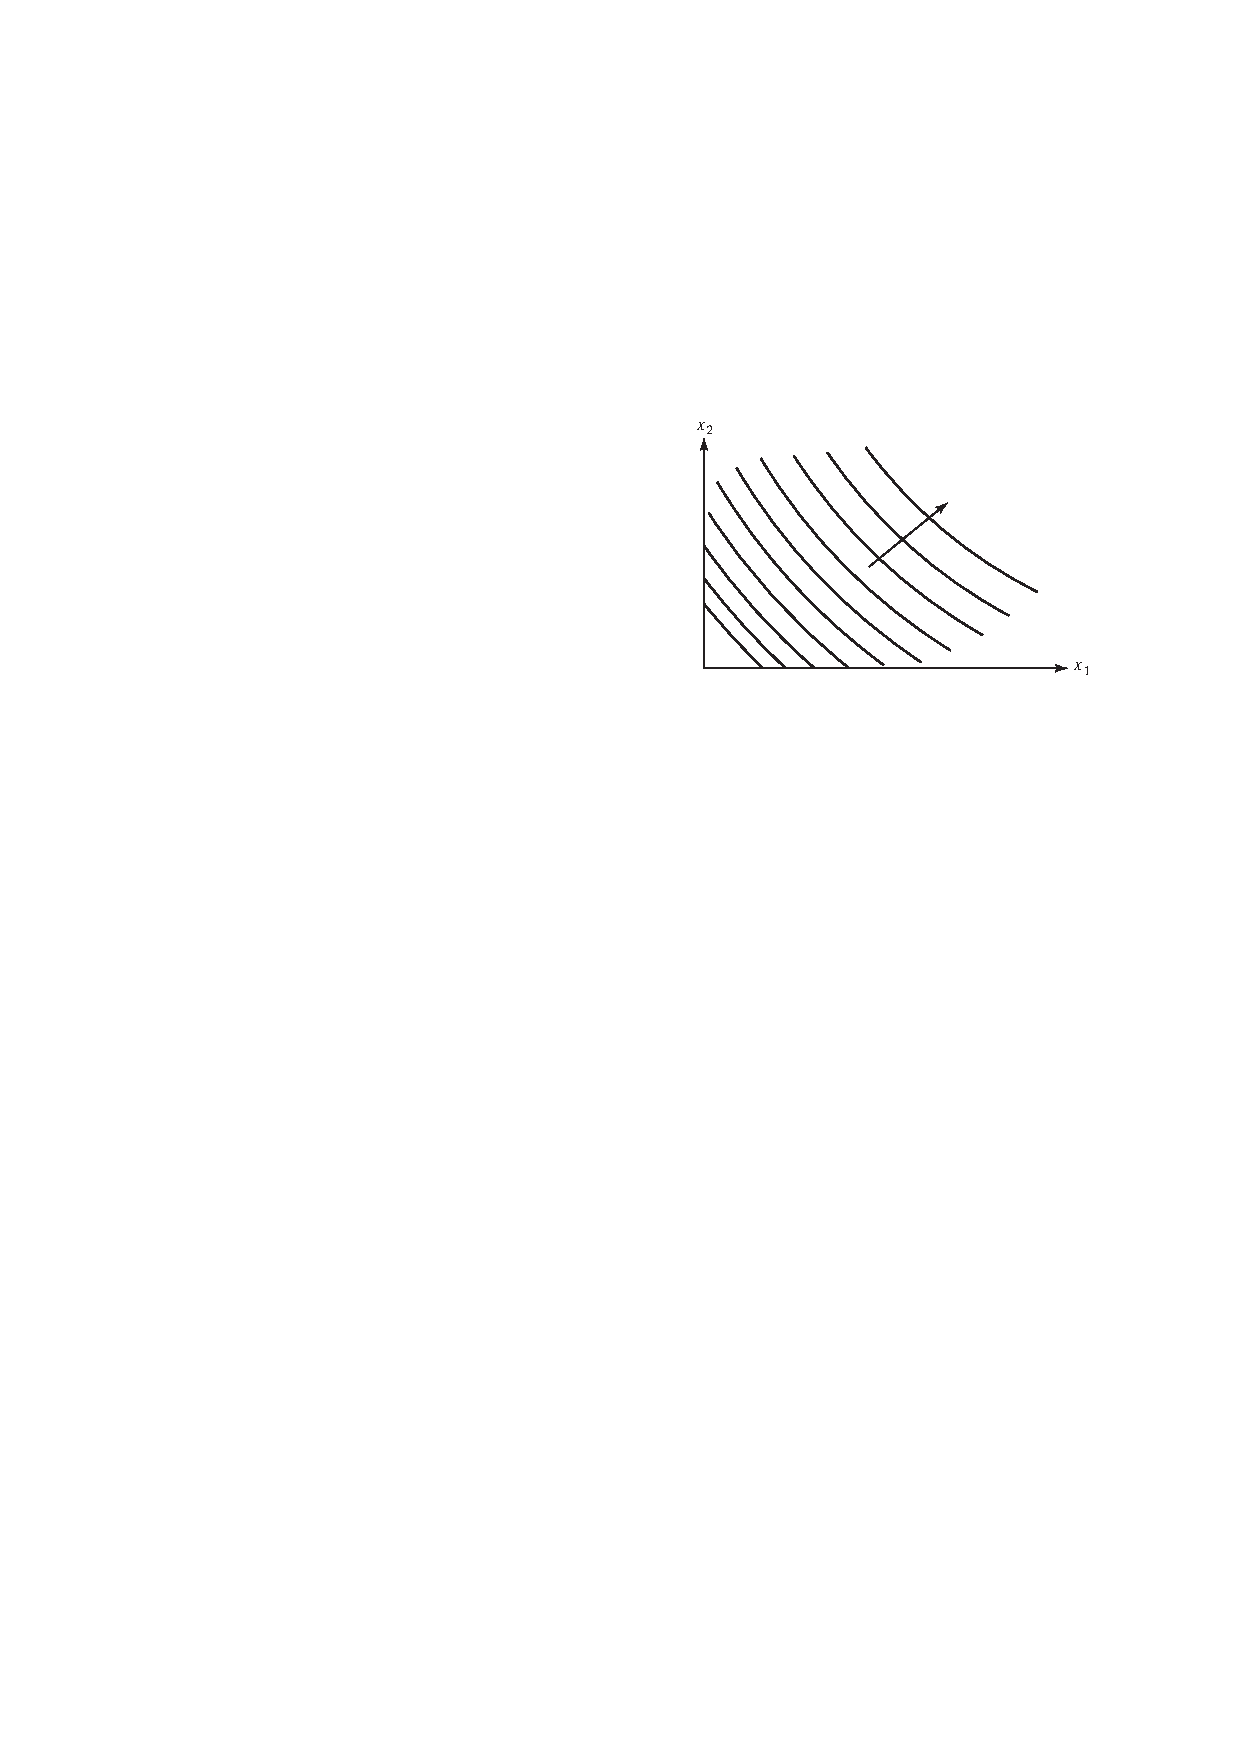
\includegraphics[width=10cm]{fig6.pdf}
  \caption{满足假设\ref{pos:pos1.2}的无差异曲线}\label{fig1.6}
\end{figure}

接下来假设消费者所处的环境是市场经济, 它是一个经济系统, 人与人之间的交易是在这一市场中进行的, 每种商品$i$都有自己的市场且价格$p_i>0$, 而且消费者在每个市场的影响力很小, 市场价格$\p\gg\mathbf{0}$是固定不变的. 消费者所处经济环境的假设可由\textbf{预算集} (budget set)表示.
\begin{definition}\label{def:def1.3}
消费者的预算集是$B=\{\x\in\R_+^n: \mathbf{p}\cdot\x\leq y\}$.
\end{definition}
在定义\ref{def:def1.3}中
$$\p\cdot\x=\sum_{i=1}^{n}p_ix_i$$
表明消费者的预算不能超过它所拥有的全部财富$y\in \R_+$. 在只有两种商品的情况下, 预算集$B$由图\ref{fig1.7}的阴影部分和边界上的消费束构成.
\begin{figure}[htbp!]
  \centering
  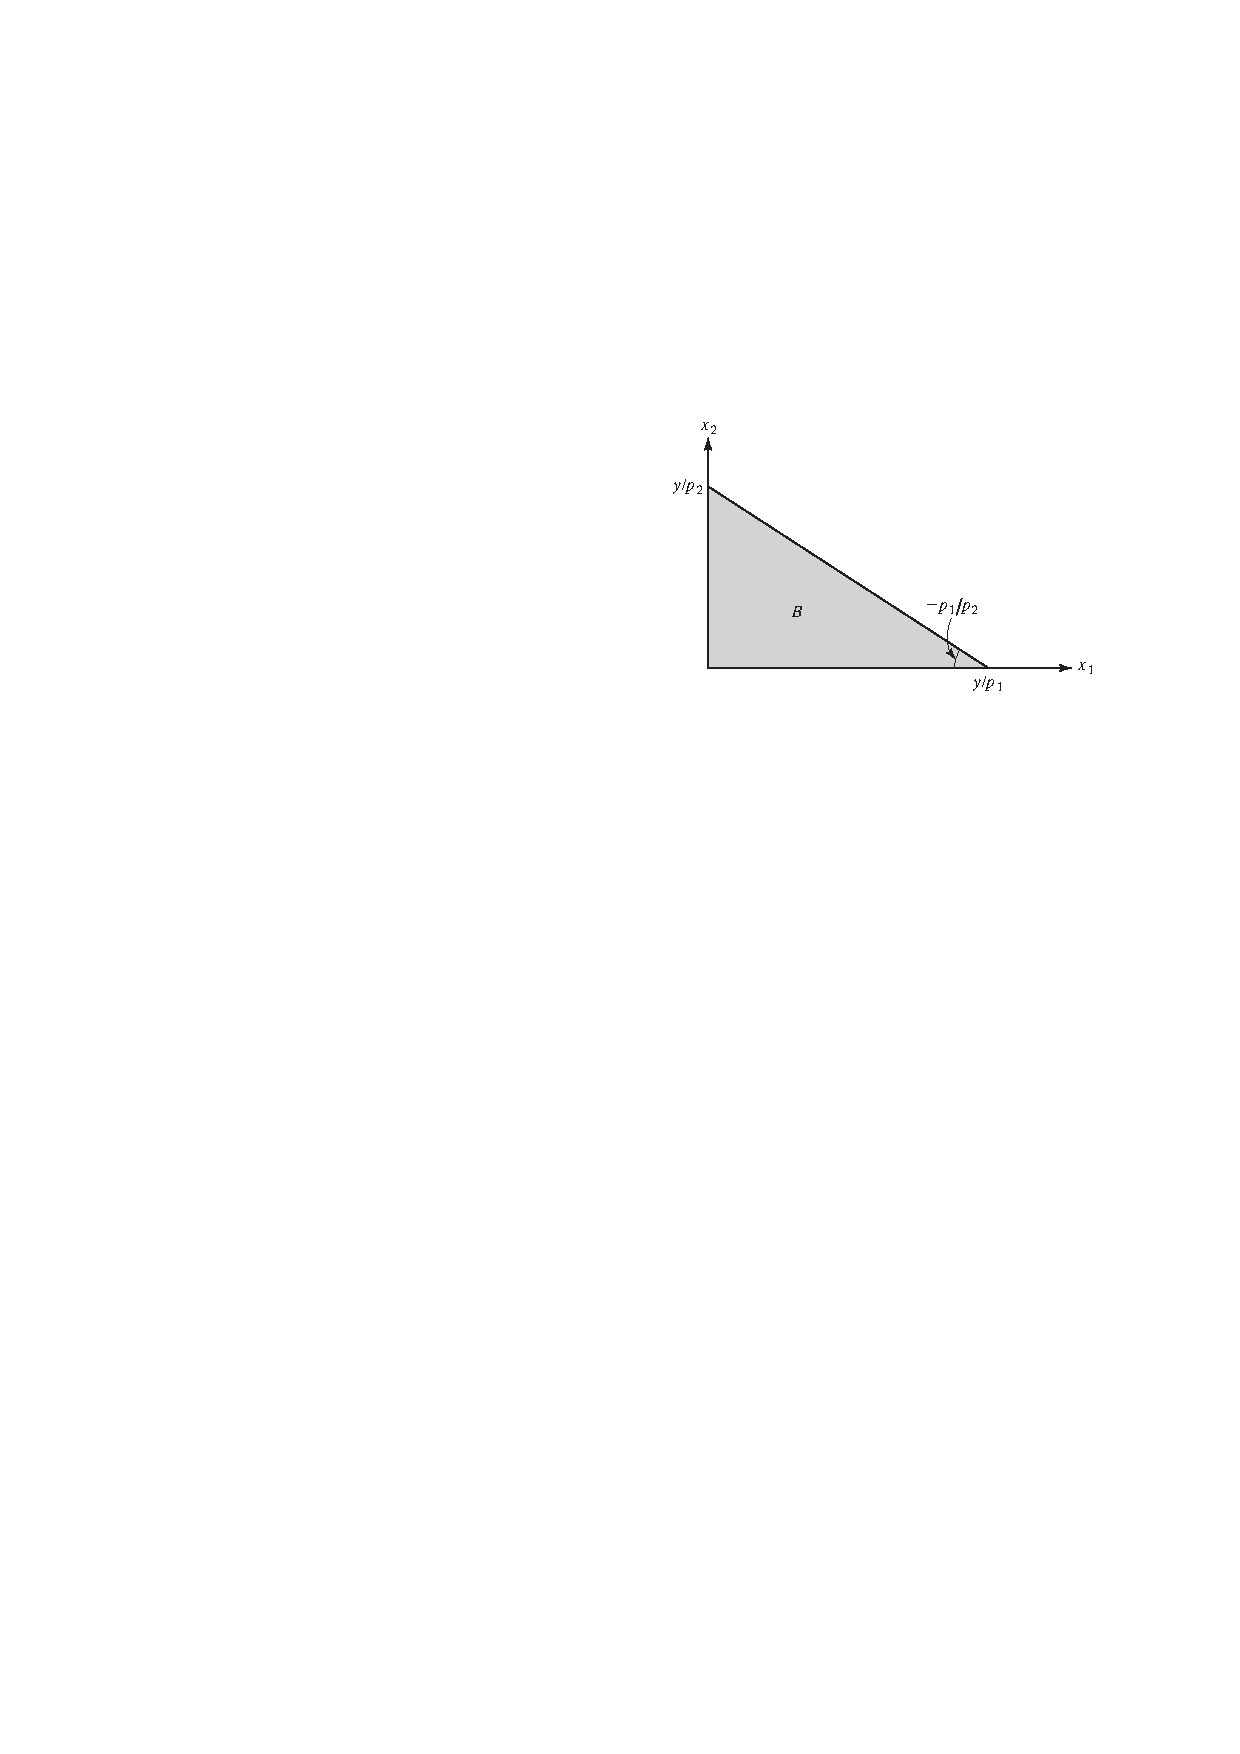
\includegraphics[width=9cm]{fig7.pdf}
  \caption{两种商品时的预算集$B=\{(x_1,x_2): p_1x_1+p_2x_2\leq y\}$.}\label{fig1.7}
\end{figure}

消费者的问题是在预算集$B$中选择一个消费束$\x^\ast$, 使得对于一切$\x\in B$都有$\x^\ast\succsim \x$. 在假设\ref{pos:pos1.2}成立的条件下, 该问题等价于预算约束下的\textbf{效用最大化问题} (Utility Maximization Problem, UMP)
\begin{equation}\label{eq1.3}
  \max_{\x\in\R^n_+} u(\x)\quad \text{s.t.}\quad \p\cdot\x\leq y
\end{equation}
\begin{proposition}\label{pro:pro1.2}
在假设\ref{pos:pos1.2}成立的条件下, UMP具有唯一解.
\end{proposition}
\begin{proof}
  假设$\p\gg\mathbf{0}$, 由于$B$是$\R^n_+$中的有界闭集, 根据Heine-Borel定理可知$B=\{\x\in\R_+^n:\p\cdot\x\leq y\}$是一个紧集, 由于$u$是连续函数, 故而$u$在$B$上具有最大值, 将最大值点记为$\x^\ast$, 假设还存在$\x^0\neq \x^\ast$为UMP的解, 根据$u$的严格拟凹性可知, 对于任意$t\in [0,1]$, 存在$\x^1=t\x^\ast+(1-t)\x^0$, 使得$u(\x^1)>u(\x^\ast)$, 这与$\x^\ast$为UMP的解矛盾, 因此$\x^\ast$是唯一的.
\end{proof}
根据命题\ref{pro:pro1.2}可知, 一旦给定了价格向量$\p$和财富水平$y$, UMP的解向量$\x^\ast$是唯一的, 可以用图\ref{fig1.8}表示.
\begin{figure}[htbp!]
  \centering
  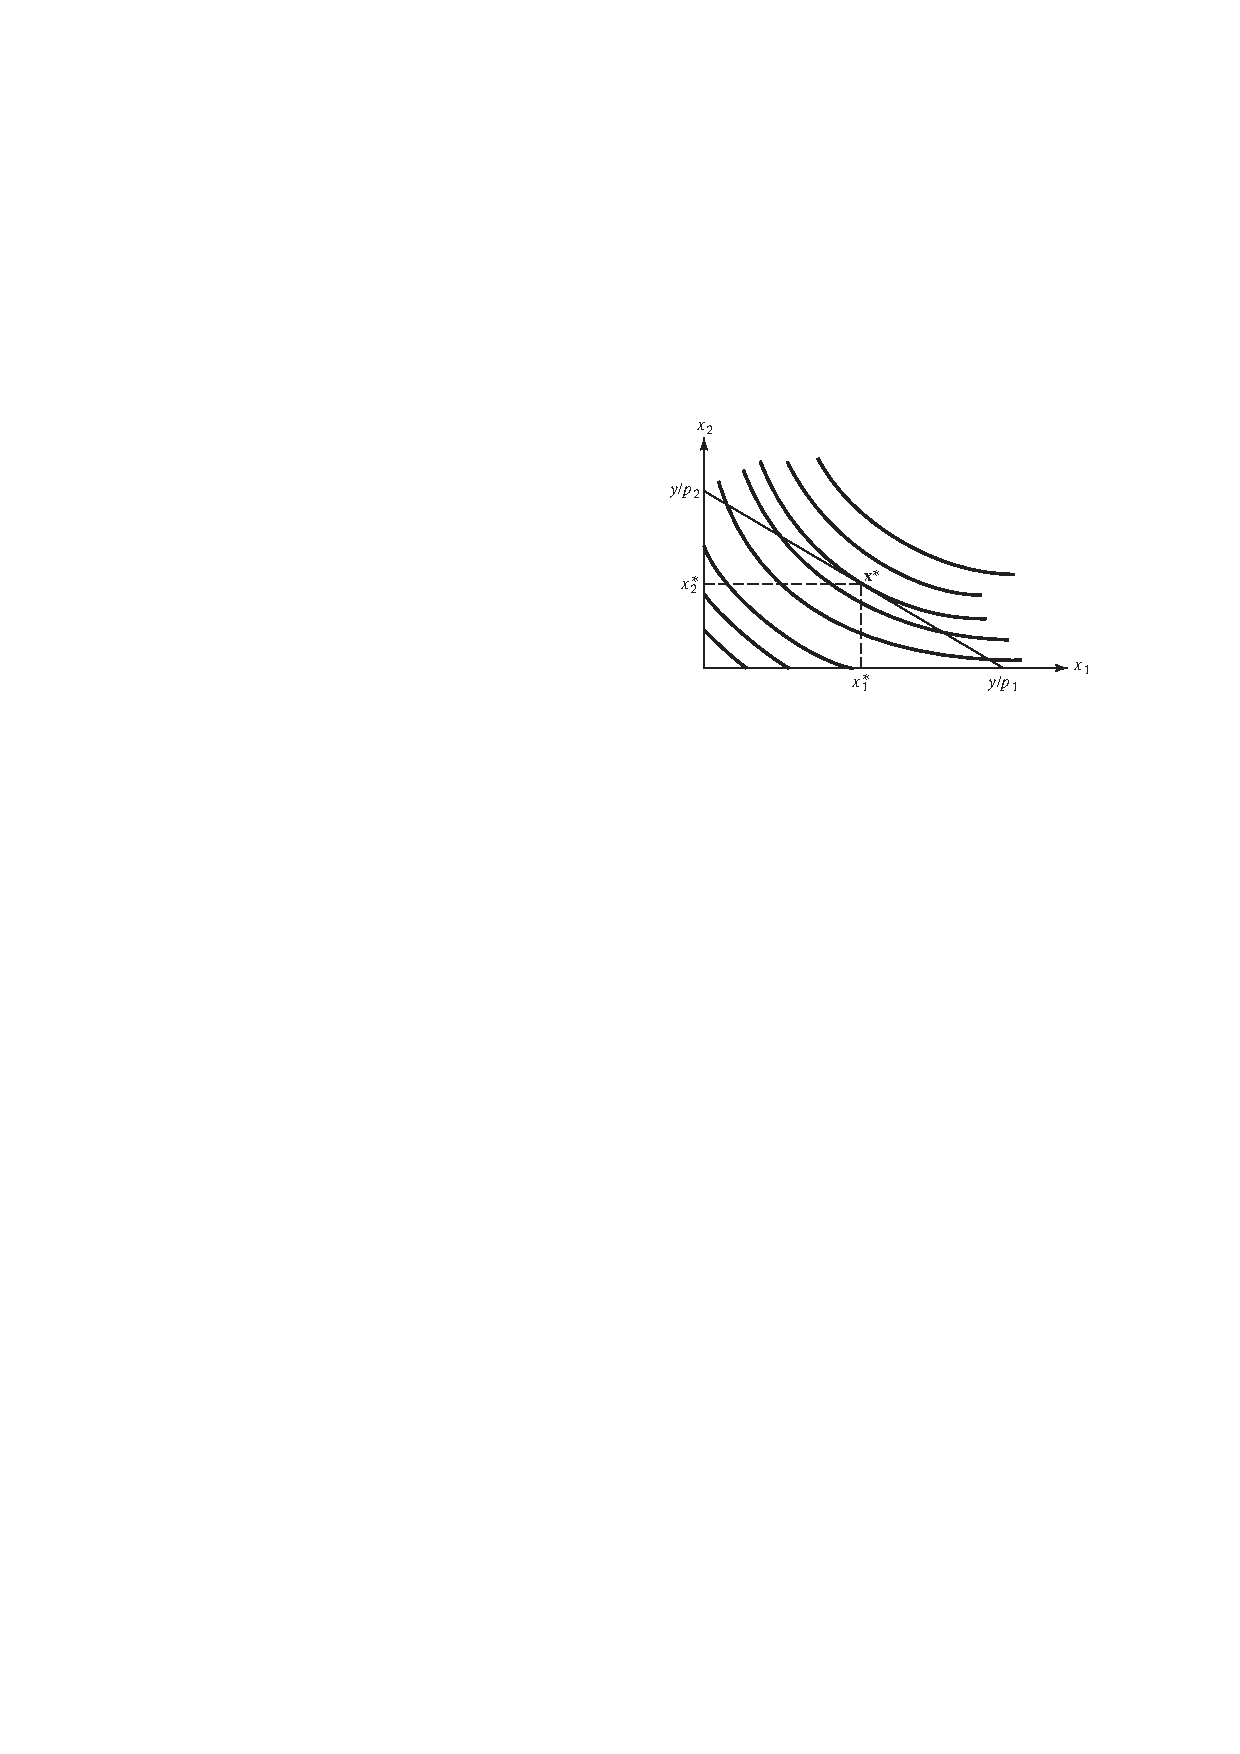
\includegraphics[width=10cm]{fig8.pdf}
  \caption{UMP的唯一解$\x^\ast$.}\label{fig1.8}
\end{figure}

另一方面, 可以将解向量记作$\x^\ast=\x(\p,y)$. 对于每个$i=1,\cdots,n$, 称$x_i^\ast=x_i(\p,y)$为Marshall需求函数. 当收入和其他商品的价格维持不变, 只有某商品自身的价格变化时, 需求量$x_i$和它自身价格$p_i$的关系图称为商品$i$的标准需求曲线. 特别地, 当只有两种商品时, 需求曲线如图\ref{fig1.9}所示: 保持商品2的价格$p_2^0$和收入水平$y$不变, 当商品1的价格从$p_1^0$下降至$p_1^1$时, 商品1的需求从$x_1(p_1^0,p_2^0,y)$上升至$x_1(p_1^1,p_2^0,y)$.
\begin{figure}[htbp!]
  \centering
  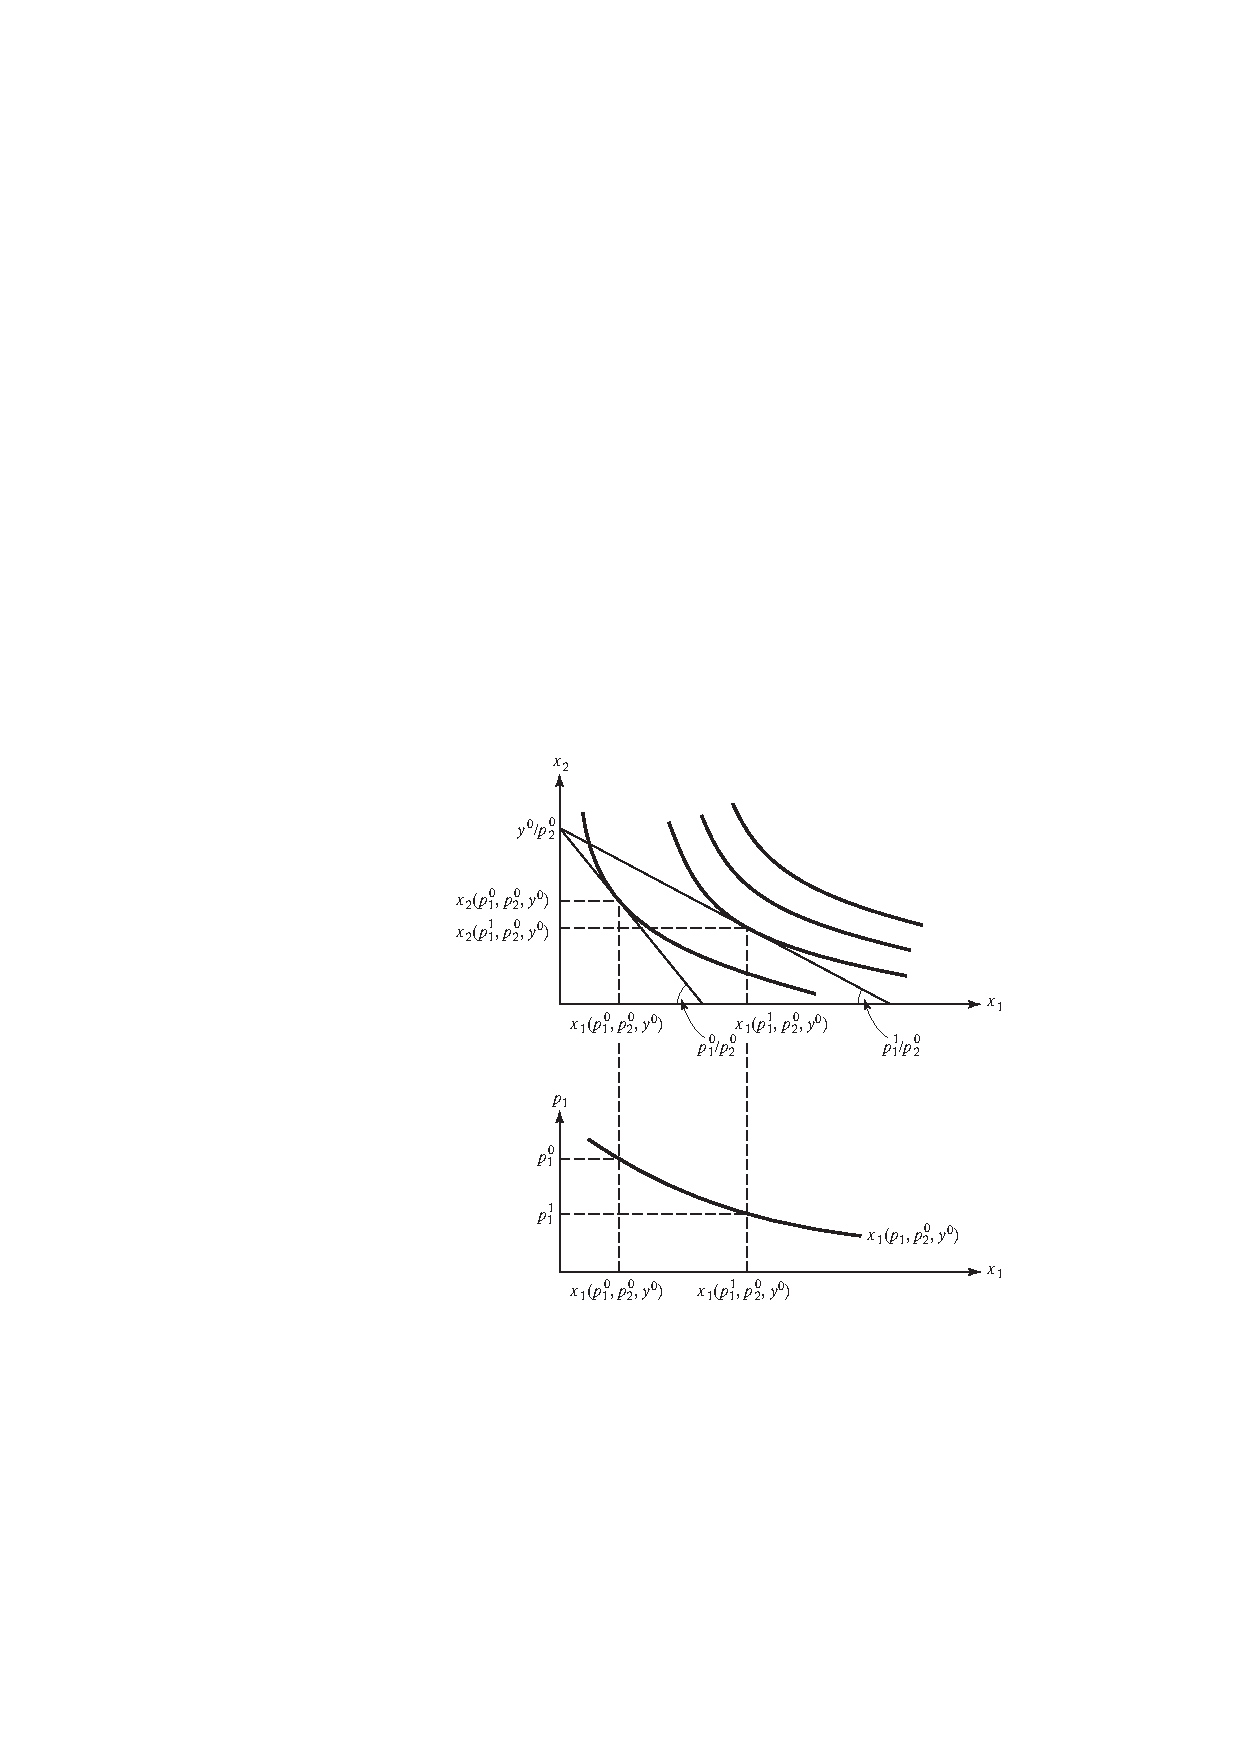
\includegraphics[width=12cm]{fig9.pdf}
  \caption{消费者需求行为.}\label{fig1.9}
\end{figure}

现在假设效用函数$u$是可微的, 回忆UMP为
\begin{equation}\label{eq1.4}
  \max_{\x\in\R^n_+} u(\x)\quad \text{s.t.}\quad \p\cdot\x\leq y
\end{equation}
前面已经指出UMP具有唯一解$\x^\ast$, 将约束条件改写为$\p\cdot\x\leq y$并构造Lagrangian函数
$$\mathcal{L}(\x,\lambda)=u(\x)-\lambda(\p\cdot\x-y)$$
其中$\lambda$为 Lagrangian乘子. 如果UMP最优解$\x^\ast\gg\mathbf{0}$, 根据Kuhn-Tucker条件可知存在$\lambda^\ast\ge0$使得$(\x^\ast,\lambda^\ast)$满足
\begin{align}
\frac{\partial\mathcal{L}}{\partial x_i}=\frac{\partial u(\x^\ast)}{\partial x_i}-\lambda^\ast p_i&=0,\,\quad i=1,\cdots, n \label{eq1.5} \\
\p\cdot\x^\ast&\leq 0  \label{eq1.6} \\
\lambda^\ast(\p\cdot\x^\ast-y)&=0 \label{eq1.7}
\end{align}
根据严格单调性可知, 为了实现消费者效用最大化, 消费者会花光全部预算$y$, 也即$\p\cdot\x^\ast=y$, 因此式(\ref{eq1.7})是多余的. 此时, 上述条件可以简化为
\begin{align}
\begin{split}
\frac{\partial\mathcal{L}}{\partial x_1}=\frac{\partial u(\x^\ast)}{\partial x_1}-\lambda^\ast p_1&=0  \\
&\vdots  \\
\frac{\partial\mathcal{L}}{\partial x_n}=\frac{\partial u(\x^\ast)}{\partial x_n}-\lambda^\ast p_n&=0 \\
\p\cdot\x^\ast&=0
\end{split}
\label{eq1.8}
\end{align}
假设$\nabla u(\x^\ast)=\mathbf{0}$, 由严格单调性可知$\partial u(\x^\ast)/\partial x_i>0$, $i=1,\cdots,n$, 从而$\partial u(\x^\ast)/\partial x_i=\lambda^\ast p_i>0$. 由此可见, 对于任意商品$i$和$j$, 在UMP的解$\x^\ast$处有
\begin{equation}\label{eq1.9}
  \text{MRS}_{ij}(\x^\ast)=\frac{\partial u(\x^\ast)/\partial x_j}{\partial u(\x^\ast)/\partial x_i}=\frac{p_j}{p_i}
\end{equation}
表明最优解$\x^\ast$处的两种商品的边际替代率必然等于这两种商品价格之比.

一般而言, 式(\ref{eq1.8})表示的一阶条件 (First Order Condition, FOC)只是局部最优解的必要条件, 但以下定理表明, FOC也是UMP全局最优解的充分条件.

\begin{theorem}
  设$u$在$\R_+^n$是连续和拟凹的, $(\p,y)\gg\mathbf{0}$, 如果$u$在$\x^\ast$处可微并且$(\x^\ast,\lambda^\ast)$是方程组(\ref{eq1.8})的解, 那么$\x^\ast$也是UMP在$(\p,y)$时的解.
\end{theorem}
\begin{proof}
  假设$\nabla u(\x^\ast)$存在且$(\x^\ast,\lambda^\ast)$是方程组(\ref{eq1.8})的解, 那么
  \begin{align*}
  \nabla u(\x^\ast)&=\lambda^\ast\p \\
  \p\cdot\x^\ast&=y
  \end{align*}
  如果$\x^\ast$不是UMP的解, 那么必然存在某个$\x^0\in \R^n_+$, 使得
  \begin{align*}
  u(\x^0)&=u(\x^\ast) \\
  \p\cdot\x^0&\leq y
  \end{align*}
  由于$u$是连续函数且$y>0$, 于是存在某个充分接近1的实数$t\in [0,1]$, 使得
  \begin{align*}
  u(t\x^0)&>u(\x^\ast) \\
  \p\cdot t\x^0&<y
  \end{align*}
  再令$\x^1=t\x^0$, 于是
  $$\nabla u(\x^\ast)(\x^1-\x^\ast)=(\lambda^\ast\p)\cdot(\x^1-\x^\ast)=\lambda^\ast(\p\cdot\x^1-\p\cdot\x^\ast)<\lambda^\ast(y-y)=0$$
  由于$u$是拟凹的且$u(\x^1)\geq u(\x^\ast)$, 于是对于任意$t\in[0,1]$都有
  $$\frac{u(t(\x^1-\x^\ast)+\x^\ast)-u(\x^\ast)}{t}\ge0$$
  当$t\to0$时取极限可得$\nabla u(\x^\ast)(\x^1-\x^\ast)\ge 0$
  这就产生了矛盾, 因此$\x^\ast$必然是UMP的解.
\end{proof}
\begin{example}
设$u(x_1,x_2)=(x_1^\rho+x_2^\rho)^{1/\rho}$, $0\ne \rho<1$, 称为CES效用函数, 容易证明它代表的偏好是严格单调和严格凸的. 考虑消费者问题
\begin{equation}\label{eq1.10}
  \max_{x_1,x_2}(x_1^\rho+x_2^\rho)^{1/\rho}\quad \text{s.t.}\quad p_1x_1+p_2x_2\leq y
\end{equation}
构造Lagrangian函数
$$\mathcal{L}(x_1,x_2,\lambda)=(x_1^\rho+x_2^\rho)^{1/\rho}-\lambda(p_1x_1+p_2x_2-y)$$
得到FOC为
\begin{align*}
\frac{\partial \mathcal{L}}{\partial x_1}&=(x_1^\rho+x_2^\rho)^{1/\rho}x_1\rho^{\rho-1}-\lambda p_1=0 \\
\frac{\partial \mathcal{L}}{\partial x_2}&=(x_1^\rho+x_2^\rho)^{1/\rho}x_2\rho^{\rho-1}-\lambda p_2=0 \\
\frac{\partial \mathcal{L}}{\partial \lambda}&=p_1x_1+p_2x_2-y=0
\end{align*}
求得UMP (\ref{eq1.10})的最优解为
\begin{align*}
x_1(p_1,p_2,y)&=\frac{p_1^{r-1}y}{p_1^r+p_2^r} \\
x_2(p_1,p_2,y)&=\frac{p_2^{r-1}y}{p_1^r+p_2^r}
\end{align*}
其中$r=\rho/(\rho-1)$.
\end{example}

\section{间接效用函数与支出}
\subsection{间接效用函数}
上面已经指出$u(\x)$是定义在消费集$X$上表示偏好关系$\succsim$的效用函数, 更具体地称为直接效用函数 (direct utility function). 给定价格向量$\p$和收入水平$y$, 消费者选择效用最大化的商品束$\x(\p,y)$, 当$\p$和$y$发生变动时, $u(\x)$的最大值也发生变动, 这可以用函数关系$v:\R_{++}^n\times \R_+\to \R$表示, $v$的定义如下
\begin{equation}\label{eq1.11}
  v(\p,y)=\max_{x\in\R_+^n}u(\x)\quad\text{s.t.}\quad\p\cdot\x\leq y
\end{equation}
称$v$为\textbf{间接效用函数} (indirect utility function), 它是UMP对应的效用最大值函数.

当$\p\gg\mathbf{0}$和$y>0$时, $v(\p,y)$是具有良好定义的函数, 因为问题(\ref{eq1.11})的解确实存在. 如果$u(\x)$是严格拟凹的, 则该问题的解唯一, 将其记作$\x(\p,y)$, 此时
$$v(\p,y)=u(\x(\p,y))$$
如图\ref{fig1.10}所示, 可以把$v(\p,y)$视作当$\p$和$y$给定时, 消费者能达到的最高无差异曲线所代表的效用水平.
\begin{figure}[htbp!]
  \centering
  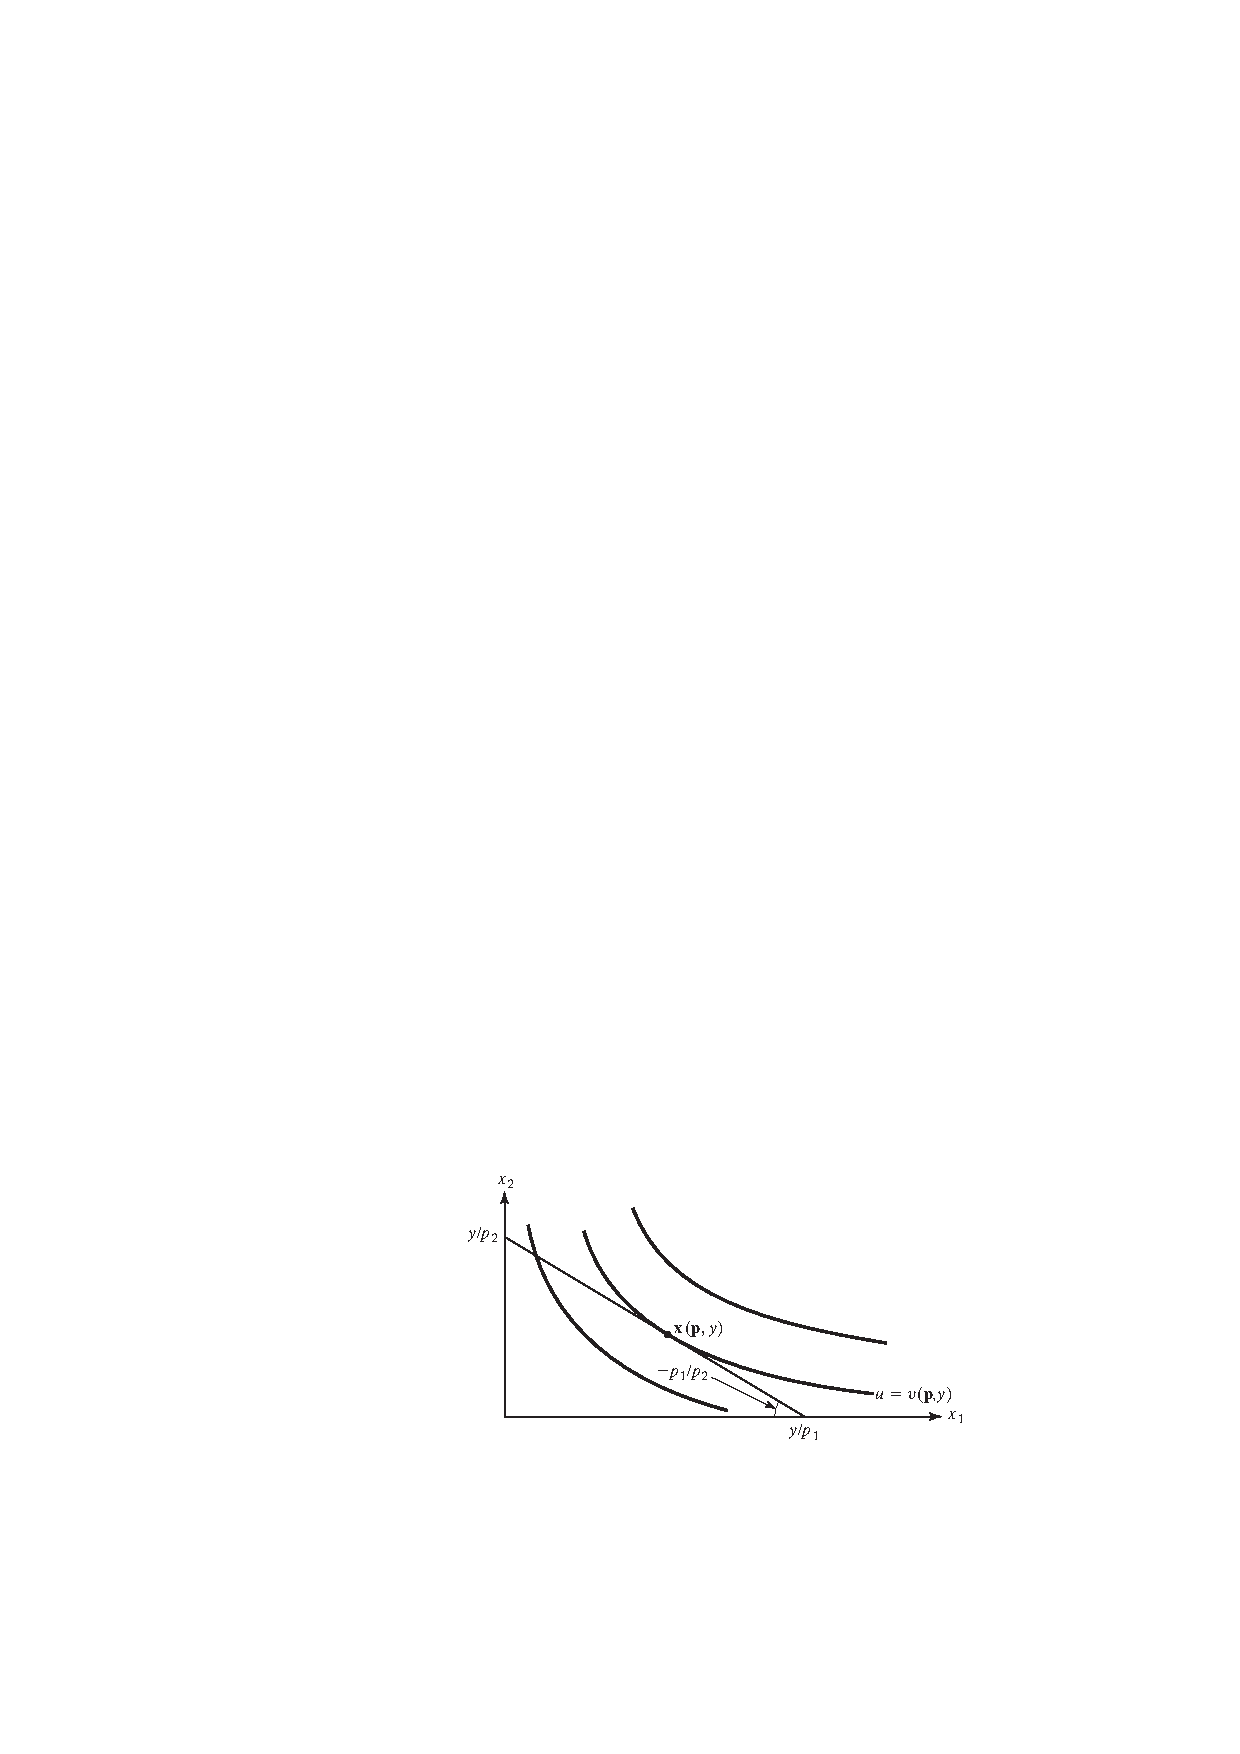
\includegraphics[width=10cm]{fig10.pdf}
  \caption{价格为$\p$收入为$y$时的间接效用函数$v(\p,y)$.}\label{fig1.10}
\end{figure}
\begin{theorem}[间接效用函数的性质]
  如果$u$在$\R_+^n$上连续且严格递增, 那么间接效用函数$v(\p,y)$具有以下性质:
  \begin{enumerate}[label=\arabic*.]
    \item 在$\R_{++}^n\times\R_+$上连续;
    \item 关于$(\p,y)$是零次齐次的;
    \item 关于$\p$是递减的;
    \item 关于$y$是递增的;
    \item 关于$(\p,y)$是拟凸的.
  \end{enumerate}
\end{theorem}
\begin{proof}
  1. 略.

  2. 对于任意$t>0$, 以下问题
  $$v(t\p,ty)=\max_{x\in\R_+^n}u(\x)\quad\text{s.t.}\quad t\p\cdot\x\leq y$$
  等价于问题(\ref{eq1.11}), 因此$v(t\p,ty)=v(\p,y)$对于$t>0$恒成立.

  3. 设$\p^0\ge\p^1$, $\x^0$是$\p=\p^0$时问题(\ref{eq1.11})的解, 因为$u$是严格递增的, 故而偏好关系$\succsim$是严格单调的, 此时约束条件变为$\p^0\cdot\x^0=y$, 故而$\p^1\cdot\x^0\leq y$, 此时消费者必然选择最优消费束$\x^1\ge \x^0$使得$\p^1\cdot\x^1=y$, 因此$v(\p^1,y)=u(\x^1)\geq u(\x^0)=v(\p^0,y)$.

  4. 设$y^0\ge y^1$, $\x^0$是$y=y^0$时问题(\ref{eq1.11})的解, 同上可知当价格水平$\p$不变时, 随着收入水平的下降, 消费者为实现$\p\cdot\x=y$, 只能将消费束缩减为$\x^1\leq \x^0$, 于是$v(\p,y^1)=u(\x^1)\leq u(\x^0)=v(\p,y^0)$.

  5. 只需证明$v$的下轮廓集$\{(\p,y):v(\p,y)\leq q\}$对于任意$q\in\R$都是凸的. 假设对于$(\p^0,y^0)$和$(\p^1,y^1)$都有$v(\p^0,y^0)\leq q$及$v(\p^1,y^1)\leq q$, 对于任意$t\in[0,1]$, 定义
  \begin{align*}
  \p^2&=t\p^0+(1-t)\p^1 \\
  y^2&=ty^0+(1-t)y^1
  \end{align*}
  现在需要证明$v(\p^2,y^2)\leq q$. 由于$v(\p^2,y^2)$是价格为$\p^2$且收入为$y^2$时$u(\x)$的最大值函数, 故而只需证明此时对一切$\x\in\R_+^n$都有$u(\x)\leq q$即可. 注意到如果$\p^2\cdot\x\leq y^2$, 那么
  $$t\p^0\cdot\x+(1-t)\p^1\cdot\x\leq ty^0+(1-t)y^1$$
  因此, 要么$\p^0\cdot \x\leq y^0$, 要么$\p^1\cdot\x\leq y^1$, 或者两者都成立. 如果$\p^0\cdot \x\leq y^0$, 那么$u(\x)\leq v(\p^0,y^0)\leq q$; 如果$\p^1\cdot\x\leq y^1$, 那么$u(\x)\leq v(\p^1,y^1)\leq q$, 结论成立.

\end{proof}
\begin{theorem}[Roy恒等式]
  如果$u$在$\R_+^n$上连续且严格递增, $v$在$(\p^0,y^0)\gg\mathbf{0}$处可微且$\partial v(\p^0,y^0)/\partial y\ne0$, 那么
  $$x_i(\p^0,y^0)=-\frac{\partial v(\p^0,y^0)/\partial p_i}{\partial v(\p^0,y^0)/\partial y},\quad i=1,\cdots,n$$
\end{theorem}
\begin{proof}
  假设$\x^0=\x(\p^0,y^0)$, 再定义$v(\p,\p\cdot\x^0)$, 于是
  $$v(\p,\p\cdot\x^0)=\max_{\x\in\R_+^n}u(\x)\text{s.t.}\quad \p\cdot\x\leq \p\cdot\x^0$$
  由于$\x^0$位于预算集内, 故而$v(\p,\p\cdot\x^0)\geq u(\x^0)=v(\p^0,\p^0\cdot\x^0)$对任意$\p\gg\mathbf{0}$成立. 再定义函数$f(\p)=v(\p,\p\cdot\x^0)$, 显然当$\p=\p^0$时, $f(\p)$在$\R_{++}^n$内取得最小值, 由于$v$在$(\p^0,y^0)$处可微, 故而$f$在$\p=\p^0$处的梯度为$\mathbf{0}$, 因此
  $$\frac{\partial f(\p^0)}{\partial \p}=\frac{\partial v(\p^0,\p^0\cdot\x^0)}{\partial \p}+\frac{\partial v(\p^0,\p^0\cdot\x^0)}{\partial (\p\cdot\x^0)}\x^0=\mathbf{0}$$
  整理即得结论.
\end{proof}
值得注意的是, 如果问题(\ref{eq1.11})的解$\x^\ast=\x(\p,y)$严格为正并且是可微的, 那么此时可以定义Lagrangian函数
$$\mathcal{L}(\x,\lambda;\p,y)=u(\x)-\lambda(\p\cdot\x-y)$$
于是$v(\p,y)$是$\mathcal{L}(\x,\lambda;\p,y)$的最优值函数, 根据\textbf{包络定理} (envelope theorem)可知在最优解$(\x^\ast,\lambda^\ast)$处有
$$\frac{\partial v(\p,y)}{\partial p_i}=\frac{\partial \mathcal{L}}{\partial p_i}=-\lambda^\ast x_i^\ast$$
以及
$$\frac{\partial v(\p,y)}{\partial y}=\frac{\partial \mathcal{L}}{\partial y}=\lambda^\ast$$
结合以上二式即可推得Roy恒等式.

\begin{example}
考虑CES效用函数$u(x_1,x_2)=(x_1^\rho+x_2^\rho)^{1/\rho}$, $0\neq\rho<1$, 于是Marshall需求函数为
$$x_1(\p,y)=\frac{p_1^{r-1}y}{p_1^r+p_2^r},\quad x_2(\p,y)=\frac{p_2^{r-1}y}{p_1^r+p_2^r}$$
其中$r=\rho/(\rho-1)$. 进一步可得间接效用函数
$$v(\p,y)=\{[x_1(\p,y)]^\rho+[x_2(\p,y)]^\rho\}^{1/\rho}=y(p_1^r+p_2^r)^{-1/r}$$
\end{example}
\subsection{支出函数}
现在我们想知道给定一组价格, 消费者能够实现既定效用水平的最小货币支出水平为多少, 如图\ref{fig1.11}所示, 预算约束线从东北往西南移动的过程中, 消费者可以选取无差异曲线上的消费束以实现既定效用水平$u$, 直观上看, 最低的预算约束线是和无差异曲线相切的那条.

事实上, 图\ref{fig1.11}中平行的\textbf{等支出线 }(isoexpenditure curve)$e=p_1x_1+p_2x_2$描述的是价格水平$\p=(p_1,p_2)$保持不变时, 在各收入水平下消费的商品束. 当支出水平低至$e^3$时, 显然消费者无法实现效用水平$u$.

\begin{figure}[htbp!]
  \centering
  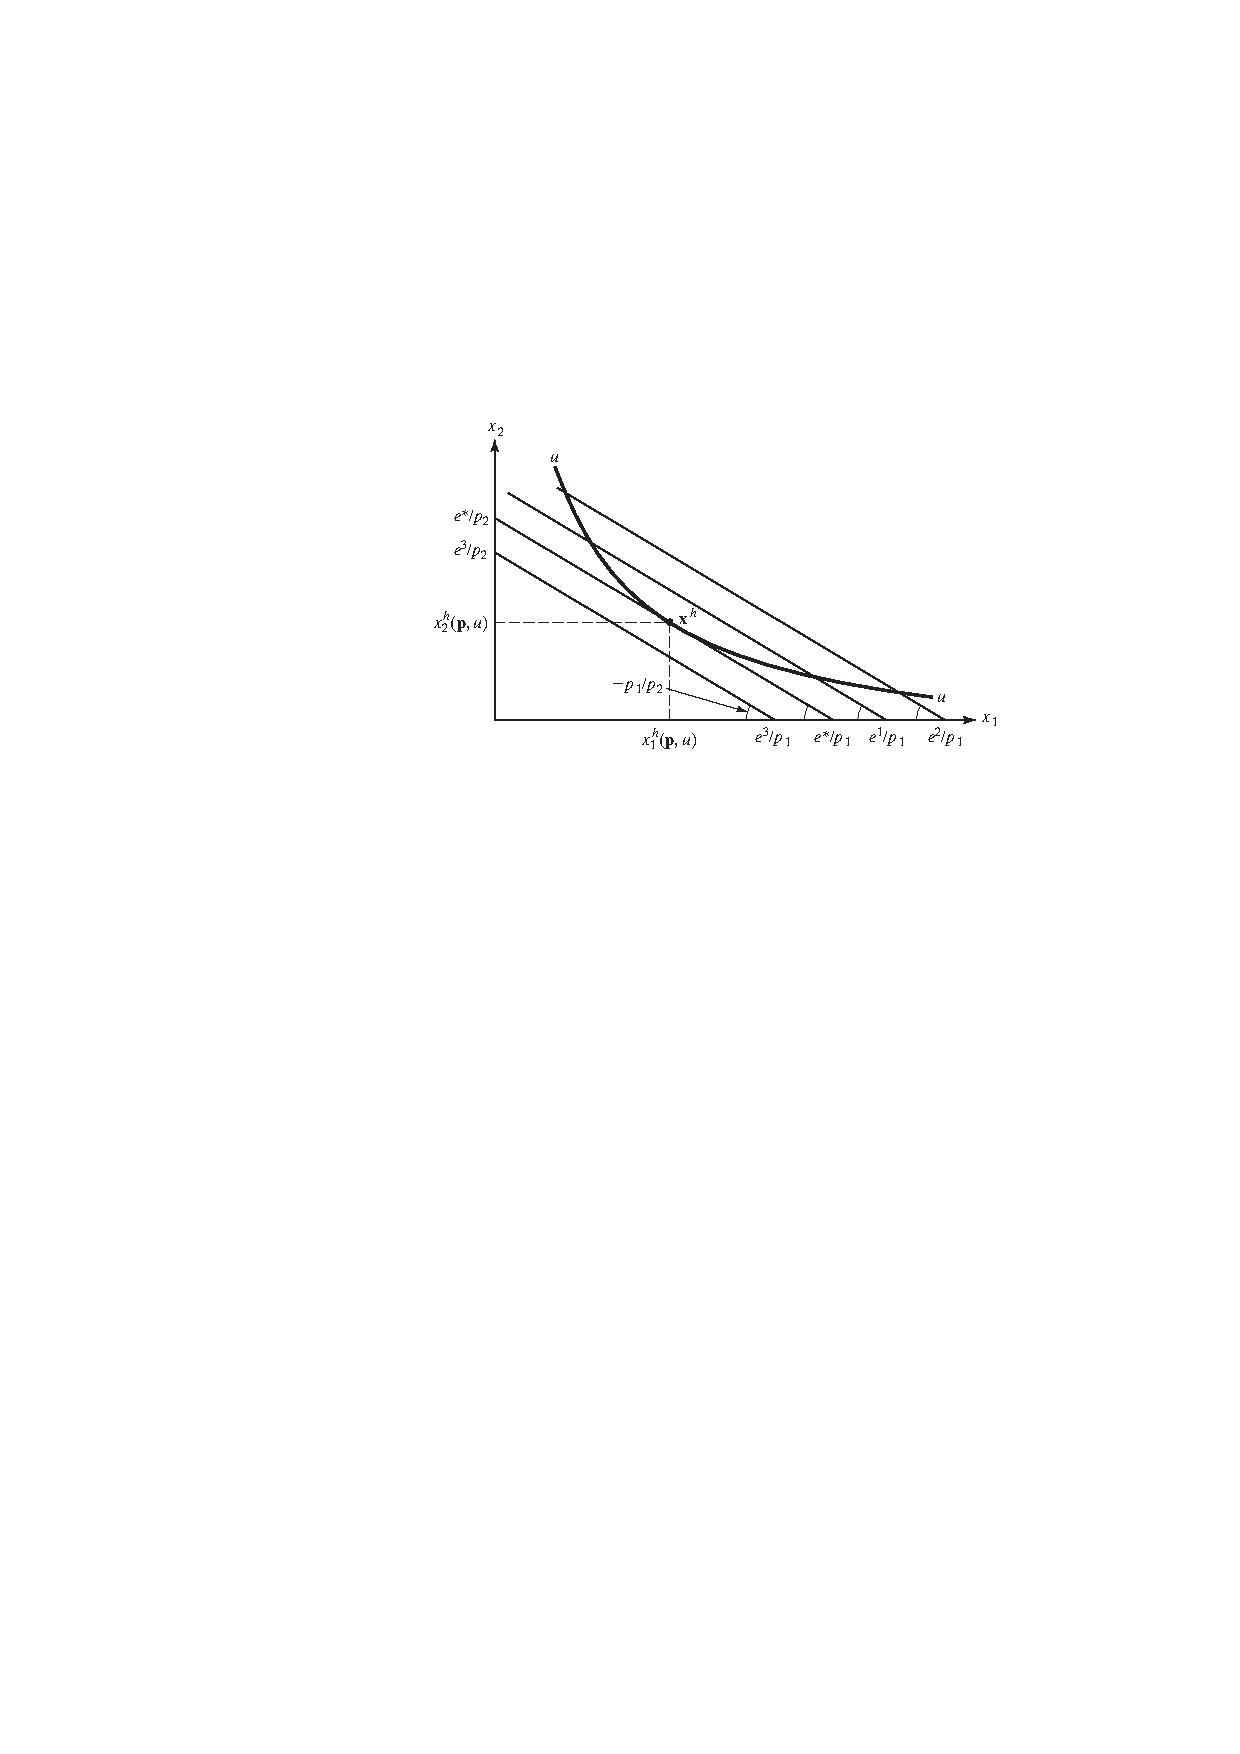
\includegraphics[width=10cm]{fig11.pdf}
  \caption{寻找最低预算水平使得消费者达到既定效用水平$u$.}\label{fig1.11}
\end{figure}

更一般地, 考虑将消费者\textbf{支出最小化问题} (Expenditure Minimization Problem, EMP)定义为
\begin{equation}\label{eq1.12}
  e(\p,u)=\min_{\x\in\R_+^n} \p\cdot\x\quad\text{s.t.}\quad u(\x)\ge u
\end{equation}
其中$e(\p,u)$称为\textbf{支出函数} (expenditure function), 方便起见, 定义$\mathcal{U}=\{u(\x):\x\in\R_+^n\}$表示可以达到的效用水平, 支出函数$e$的定义域为$\R_{++}^n\times\mathcal{U}$.

支出函数$e(\p,u)$的定义是良好的, 这是因为对于任意$\p\gg\mathbf{0}$和$\x\in\R_+^n$, 集合$\{e=\p\cdot\x: u(\x)\geq u\}$存在下界0, 还可以证明它是闭集, 因而它有最小值, 这个最小值就是$e(\p,u)$.

EMP的任意解向量都非负且取决于$(\p,u)$, 如果效用函数$u$是连续和严格拟凹的, 那么解唯一. 如果$\x^h(\p,u)$是EMP的解, 那么它表示价格水平为$\p$时, 为使消费者达到效用水平$u$的最小支出恰好等于消费商品束$\x^h(\p,u)$的支出, 也即$e(\p,u)=\p\cdot\x^h(\p,u)$. 事实上, 对于特定的商品$i$而言, $x_i^h(\p,u)$又称为Hicks需求函数或补偿需求函数.

如图\ref{fig1.12}所示, 维持商品2的价格$p_2^0$不变, 当商品1的价格从$p_1^0$下降到$p_1^1$时, 为使消费者获得相同的效用$u$且实现最小支出, 应将等支出线沿着它和无差异曲线的切点移动, 此时商品1的消费量从$x_1^h(p_1^0,p_2^0,u)$上升为$x_1^h(p_1^1,p_2^0,u)$, 这样一直做下去即可得到商品1的Hicks需求曲线. 显然, 效用水平不同Hicks需求曲线也不同, 但它的形状和位置总取决于消费者的偏好.
\begin{figure}[htbp!]
  \centering
  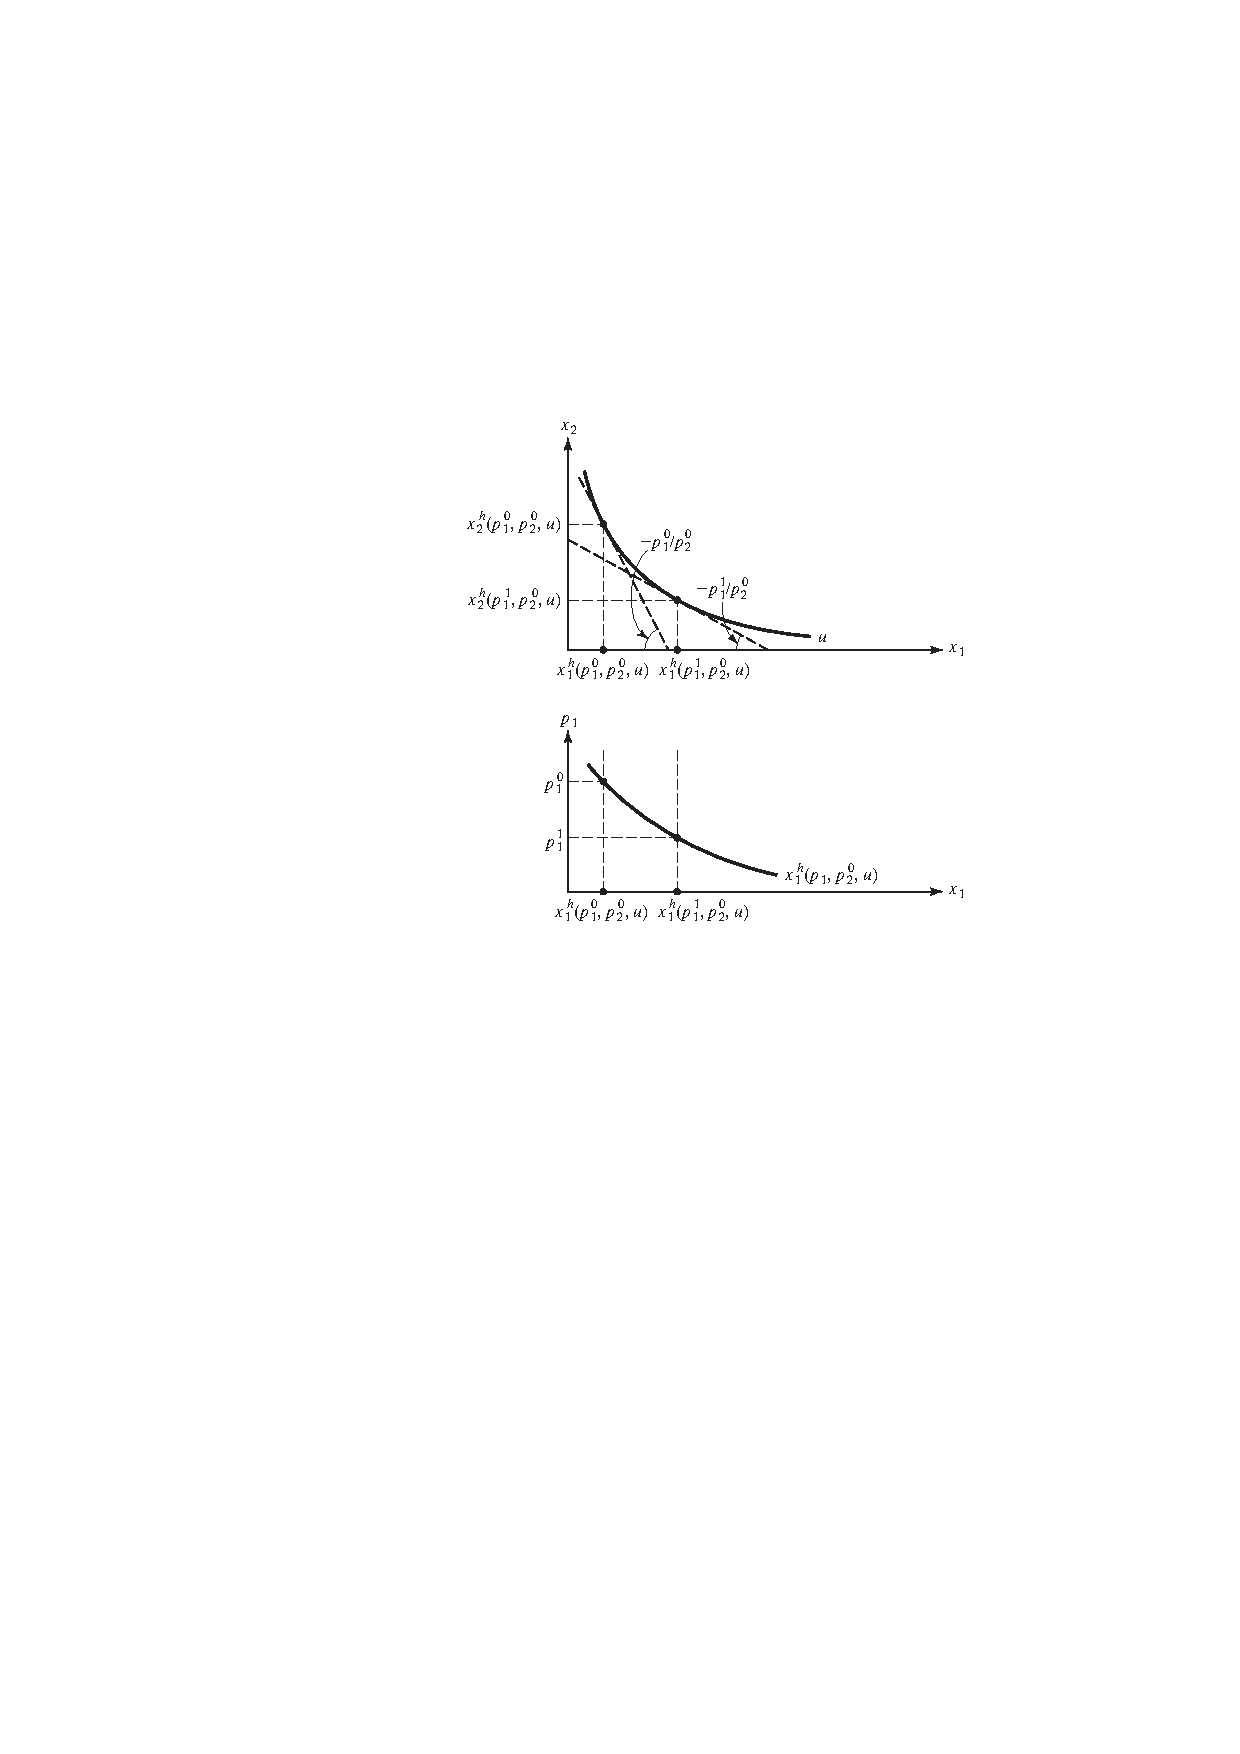
\includegraphics[width=10cm]{fig12.pdf}
  \caption{商品1的Hicks需求函数.}\label{fig1.12}
\end{figure}

\begin{theorem}[支出函数的性质]
  如果$u$在$\R_+^n$上连续且严格递增, 那么支出函数$e(\p,u)$具有以下性质:
  \begin{enumerate}[label=\arabic*.]
    \item 在$\R_{++}^n\times\mathcal{U}$上连续;
    \item 关于$u$是递增的;
    \item 关于$\p$是递增的;
    \item 关于$\p$是一次齐次的;
    \item 关于$\p$是凹函数.
  \end{enumerate}
\end{theorem}
\begin{proof}
  1. 略.

  2. 假设$e$关于$u$不是递增的, 设$\x^0$和$\x^1$分别为效用水平为$u^0$和$u^1$时的最优消费束, 并且$u^1>u^0$, $\p\cdot\x^0\geq \p\cdot\x^1>0$. 设$t\in[0,1]$为充分接近1的某个数, $\x^2=t\x^1$, 由于效用函数$u$是连续的, 故而$u(\x^2)>u^0$且$\p\cdot\x^0>\p\cdot\x^2$, 但这与$\x^0$是既定效用水平为$u^0$时的最优消费束这一事实矛盾.

  3. 假设$\p^0\ge\p^1$, $\x^0$是价格为$\p^0$时EMP的最优解, 于是
  $$e(\p^0,u)=\p^0\cdot\x^0\ge \p^1\cdot\x^0\ge e(\p^1,u)$$
  其中最后一个不等号是由$e(\p^1,u)$的定义得到的.

  4. 当价格变化时, EMP的约束集不会发生变化, 对于任意$t\ge0$, 在约束集上使$t\p\cdot\x$最小化的消费束和使$\p\cdot\x$最小化的消费束是一致的, 将其记作$\x^\ast$, 于是$e(t\p,u)=t\p\cdot\x^\ast=te(\p,u)$.

  5. 固定目标效用水平$u$, 对任意$t\in(0,1)$, 定义$\p^2=t\p^0+(1-t)\p^1$, $\x^2$是价格为$\p^2$时的EMP最优消费束, 于是
  \begin{align*}
  e(\p^2,u)&=\p^2\cdot\x^2 \\
  &=t\p^0\cdot\x^2+(1-t)\p^1\cdot\x^2 \\
  &\geq te(\p^0,u)+(1-t)e(\p^1,u)
  \end{align*}
  也即$e$关于$\p$是凹的.
\end{proof}

\begin{theorem}[Shephard引理]
  如果$u$在$\R_+^n$上连续且严格递增, 并且是严格拟凹的, 那么$e$在$(\p^0,u^0)$处关于$\p\gg\mathbf{0}$可微, 并且
  $$x_i^h(\p^0,u^0)=\frac{\partial e(\p^0,u^0)}{\partial p_i},\quad i=1,\cdots,n$$
\end{theorem}
\begin{proof}
  设$\p^0\gg\mathbf{0}$并且$\x^0=\x^h(\p^0,u^0)$, 于是
  $$e(\p,u^0)=\min_{\x\in\R_+^n}\p\cdot\x\quad\text{s.t.}\quad u(\x)\ge u^0$$
  也即$e(\p,u^0)$是价格为$\p$且既定效用水平为$u^0$时的最小支出, 而$\x^0=\x^h(\p^0,u^0)$也是可以实现既定效用水平$u^0$的消费束, 故而对于一切$\p\gg\mathbf{0}$都有$e(\p,u^0)\leq \p\cdot\x^0$.

  定义函数$f(\p)=e(\p,u^0)-\p\cdot\x^0$, 当且仅当$\p=\p^0$时$f$在$\R_{++}^n$上有最大值, 根据可微性可知
  $$\frac{\partial f(\p^0)}{\partial \p}=\frac{\partial e(\p^0,u^0)}{\partial \p}-\x^0=\mathbf{0}$$
  结论成立.
\end{proof}
\begin{example}
考虑CES效用函数$u(x_1,x_2)=(x_1^\rho+x_2^\rho)^{1/\rho}$, $0\neq\rho<1$, 现在来推导Hicks需求函数$\x^h(\p,u)$与支出函数$e(\p,u)$. 由于偏好关系$\succsim$是严格单调的, 故而将EMP写为
$$\min_{(x_1,x_2)\in\R_+^2}p_1x_1+p_2x_2\quad\text{s.t.}\quad u=(x_1^\rho+x_2^\rho)^{1/\rho}$$
首先定义Lagrangian函数
$$\mathcal{L}(x_1,x_2,\lambda)=p_1x_1+p_2x_2-\lambda[(x_1^\rho+x_2^\rho)^{1/\rho}-u]$$
于是
\begin{align*}
\frac{\partial\mathcal{L}}{\partial x_1}&=p_1-\lambda(x_1^\rho+x_2^\rho)^{1/\rho-1}x_1^{\rho-1}=0 \\
\frac{\partial\mathcal{L}}{\partial x_2}&=p_2-\lambda(x_1^\rho+x_2^\rho)^{1/\rho-1}x_2^{\rho-1}=0 \\
\frac{\partial\mathcal{L}}{\partial\lambda}&=(x_1^\rho+x_2^\rho)^{1/\rho}-u
\end{align*}
消去$\lambda$后可得包含两个未知数的方程
\begin{align}
x_1&=x_2\left(\frac{p_1}{p_2}\right)^{1/(\rho-1)} \label{eq1.13} \\
u&=(x_1^\rho+x_2^\rho)^{1/\rho} \label{eq1.14}
\end{align}
将式(\ref{eq1.13})代入(\ref{eq1.14})得到
$$  u=\left[x_2^\rho\left(\frac{p_1}{p_2}\right)^{\rho/(\rho-1)}+x_2^\rho\right]^{1/\rho}=x_2\left[\left(\frac{p_1}{p_2}\right)^{\rho/(\rho-1)}+1\right]^{1/\rho}
$$
再令$r=\rho/(\rho-1)$, 得到
\begin{equation}\label{eq1.15}
  x_2^h(\p,u)=u(p_1^r+p_2^r)^{1/r-1}p_2^{r-1}
\end{equation}
将式(\ref{eq1.15})代入(\ref{eq1.13})得到
$$  x_1^h(\p,u)=u(p_1^r+p_2^r)^{1/r-1}p_1^{r-1}
$$
从而支出函数为
\begin{align*}
e(\p,u)&=p_1x_1^h(\p,u)+p_2x_2^h(\p,u)=u(p_1^r+p_2^r)^{1/r}
\end{align*}
\end{example}
\subsection{间接效用函数和支出函数之间的关系}
首先固定$(\p,y)$并且令$u=v(\p,y)$, 该式表明当价格为$\p$时, $u$是消费者在收入水平为$y$时可以达到的最大效用水平. 因此, 如果消费者希望至少达到效用水平$u$, 则收入$y$应该足够大才能达到效用水平$u$, 而$e(\p,u)$是为了达到效用水平$u$所需要的最小必要支出, 于是
\begin{equation}\label{eq1.16}
  e(\p,v(\p,y))\leq y,\quad\forall (\p,y)\gg\mathbf{0}
\end{equation}
现在固定$(\p,u)$并且令$y=e(\p,u)$, 该式表明当价格为$\p$时, $y$是消费者达到既定效用水平$u$时的最小必要支出. 因此, 当价格为$\p$时, 如果消费者的收入为$y$, 那么他至少可以达到效用水平$u$, 而$v(\p,y)$是收入水平为$y$时的最大效用水平, 于是
\begin{equation}\label{eq1.17}
  v(\p,e(\p,u))\geq u,\quad\forall(\p,u)\in\R_{++}^n\times\mathcal{U}
\end{equation}
下面的定理表明, 如果对偏好关系施加一些熟悉的条件, 上述两个不等式必定成为等式.

\begin{theorem}\label{thm:thm1.3}
  设$v(\p,y)$和$e(\p,u)$分别为某个消费者的间接效用函数和支出函数, 而且该消费者的效用函数为连续且严格递增的, 那么对于一切$y\ge0$以及$(\p,u)\in\R_{++}^n\times\mathcal{U}$都有
  \begin{enumerate}[label=\arabic*.]
    \item $e(\p,v(\p,y))=y$;
    \item $v(\p,e(\p,u))=u$.
  \end{enumerate}
\end{theorem}
\begin{proof}
  因为$u$在$X=\R_+^n$上是严格递增的, 它在$\x=\mathbf{0}$处取得最小值, 但没有最大值. 又因为$u$是连续函数, 集合$\mathcal{U}$必定是一个区间, 所以对于$\overbar{u}>u(\mathbf{0})$有$\mathcal{U}=[u(\mathbf{0}),\overbar{u}]$, 其中$\overbar{u}$可以是有限的也可以是$\infty$.

  1. 固定$(\p,y)\in\R_{++}^n\times\R_+$, 只需证明式(\ref{eq1.16})只能取等号. 假设不是这样, 也即$e(\p,u)<y$, $u=v(\p,y)$, 根据$v$的定义可知$u\in\mathcal{U}$并且$u<\overbar{u}$. 根据支出函数$e$的连续性, 可以选择充分小的$\epsilon>0$使得$u+\epsilon<\overbar{u}$并且$e(\p,u+\epsilon)<y$.

  再令$y_\epsilon=e(\p,u+\epsilon)$, 于是$v$关于$y$的单调性以及式(\ref{eq1.17})意味着
  $$v(\p,y)>v(\p,y_\epsilon)\geq u+\epsilon$$
  然而$u=v(\p,y)$, 这就表明$u\ge u+\epsilon$, 产生矛盾.

  2. 固定$(\p,u)\in\R_{++}^n\times [u(\mathbf{0}),\overbar{u}]$, 同样使用反证法. 假设$v(\p,e(\p,u))>u$, 当$u=u(\mathbf{0})$时, $e(\p,u)=0$, 从而$v(\p,0)=u(\mathbf{0})$, 此时$v(\p,e(\p,u))=u$成立.

  再令$y=e(\p,u)>0$, 由于$v$是连续函数, 故而可以选取充分小的$\epsilon>0$使得$y-\epsilon>0$且$v(\p,y-\epsilon)>u$, 因此当价格为$\p$时, 只需将收入水平维持在$y-\epsilon$就可以实现比$u$更大的效用, 也即$e(\p,u)\leq y-\epsilon$, 但这与$y=e(\p,u)$矛盾.
\end{proof}

\begin{example}
考虑CES效用函数$u(x_1,x_2)=(x_1^\rho+x_2^\rho)^{1/\rho}$, $0\neq\rho<1$, 它的间接效用函数为
$$v(\p,y)=y(p_1^r+p_2^r)^{1/r}$$
其中$r=\rho/(\rho-1)$. 设$e(\p,u)=y$, 于是
\begin{equation}\label{eq1.18}
  v(\p,e(\p,u))=e(\p,u)(p_1^r+p_2^r)^{1/r}
\end{equation}
根据定理\ref{thm:thm1.3}可知对于任意$\p\gg\mathbf{0}$和$u\in\mathcal{U}$都有
\begin{equation}\label{eq1.19}
  v(\p,e(\p,u))=u
\end{equation}
联立式(\ref{eq1.18})和(\ref{eq1.19})可得
$$e(\p,u)(p_1^r+p_2^r)^{-1/r}=u$$
从上式即可解得支出函数$e(\p,u)=u(p_1^r+p_2^r)^{1/r}$.

类似地, 从$e(\p,u)=u(p_1^r+p_2^r)^{1/r}$, $u=v(\p,y)$以及$e(\p,v(\p,y))=y$可以解得间接效用函数$v(\p,y)=y(p_1^r+p_2^r)^{1/r}$.
\end{example}

\begin{theorem}[对偶关系]\label{thm:thm1.4}
  在假设\ref{pos:pos1.2}成立的条件下, 对于一切$y\ge0$及$(\p,u)\in\R_{++}^n\times\mathcal{U}$都有
  \begin{enumerate}[label=\arabic*.]
    \item $x_i(\p,y)=x_i^h(\p,v(\p,y))$;
    \item $x_i^h(\p,u)=x_i(\p,e(\p,u))$.
  \end{enumerate}
\end{theorem}
\begin{proof}
  1. 令$\x^0=\x(\p^0,y^0)$, $u^0=u(\x^0)$, 根据$v$的定义可知$v(\p^0,y^0)=u^0$以及$\p^0\cdot\x^0=y^0$, 根据定理\ref{thm:thm1.3}可知$e(\p^0,v(\p^0,y^0))=y^0$, 也即$e(\p^0,u^0)=y^0$. 另一方面, 由于$u^0=u(\x^0)$, $\p^0\cdot\x^0=y^0$, 这意味着当$(\p,u)=(\p^0,u^0)$时, $\x^0$是EMP的解, 因此$\x^0=\x^h(\p^0,u^0)$, 从而$\x(\p^0,y^0)=\x^h(\p^0,v(\p^0,y^0))$.

  2. 令$\x^0=\x^h(\p^0,u^0)$, $\p^0\cdot\x^0=y^0$, 由$e$的定义可知$e(\p^0,u^0)=y^0$以及$u^0=u(\x^0)$, 根据定理\ref{thm:thm1.3}可知$v(\p^0,e(\p^0,u^0))=u^0$, 也即$v(\p^0,y^0)=u^0$, 因此当$(\p,y)=(\p^0,y^0)$时, $\x^0$是UMP的解, 从而$\x^h(\p^0,u^0)=\x(\p^0,y^0)$.
\end{proof}
定理\ref{thm:thm1.4}表明, 当假设\ref{pos:pos1.2}的条件满足时, UMP的解同时也是EMP的解, 此时称最优解$\x^0$具有\textbf{对偶} (dual)性质.
\begin{example}
现在利用CES效用函数来验证定理\ref{thm:thm1.4}, 它的间接效用函数$v(\p,y)$和Hicks需求函数$x_i^h(\p,u)$分别为
\begin{align*}
v(\p,y)&=y(p_1^r+p_2^r)^{1/r} \\
 x_i^h(\p,u)&=u(p_1^r+p_2^r)^{1/r-1}p_i^{r-1},\quad i=1,2
\end{align*}
使用$v(\p,y)$替代$u$可得
\begin{equation}\label{eq1.20}
  x_i^h(\p,u)=\frac{yp_i^{r-1}}{p_1^r+p_2^r},\quad i=1,2
\end{equation}
类似地, 支出函数$e(\p,u)$和Marshall需求函数$x_i(\p,y)$分别为
\begin{align*}
e(\p,u)&=u(p_1^r+p_2^r)^{1/r} \\
x_i(\p,y)&=\frac{yp_i^{r-1}}{p_1^r+p_2^r},\quad i=1,2
\end{align*}
使用$e(\p,u)$代替$y$可得
\begin{equation}\label{eq1.21}
  x_i(\p,y)=up_i^{r-1}(p_1^r+p_2^r)^{1/r-1},\quad i=1,2
\end{equation}
这就表明式(\ref{eq1.20})推导出了Marshall需求函数, 而式(\ref{eq1.21})推导出了Hicks需求函数, 它们与之前UMP和EMP推导出的结论相同.
\end{example}

图\ref{fig1.13}描述了定理\ref{thm:thm1.3}和\ref{thm:thm1.4}. 当价格为$\p$且收入为$y$时, 消费者通过选择最优消费束$x_1^\ast$和$x_2^\ast$达到了最大效用$u$, 可以将其视为给定的效用水平$v(\p,y)$, 点$(p_1,x^\ast_1)$将位于商品1的Marshall需求函数上.

接下来考虑消费者EMP, 假设寻找的是达到效用水平$u$的最小支出, 显然当价格为$\p$时, EMP的最低等支出线和UMP最大预算约束线重合, 而且EMP的选择也是$x_1^\ast$和$x_2^\ast$, 从而$(p_1,x_1^\ast)$位于商品1的Hicks需求曲线上.
\begin{figure}[htbp!]
  \centering
  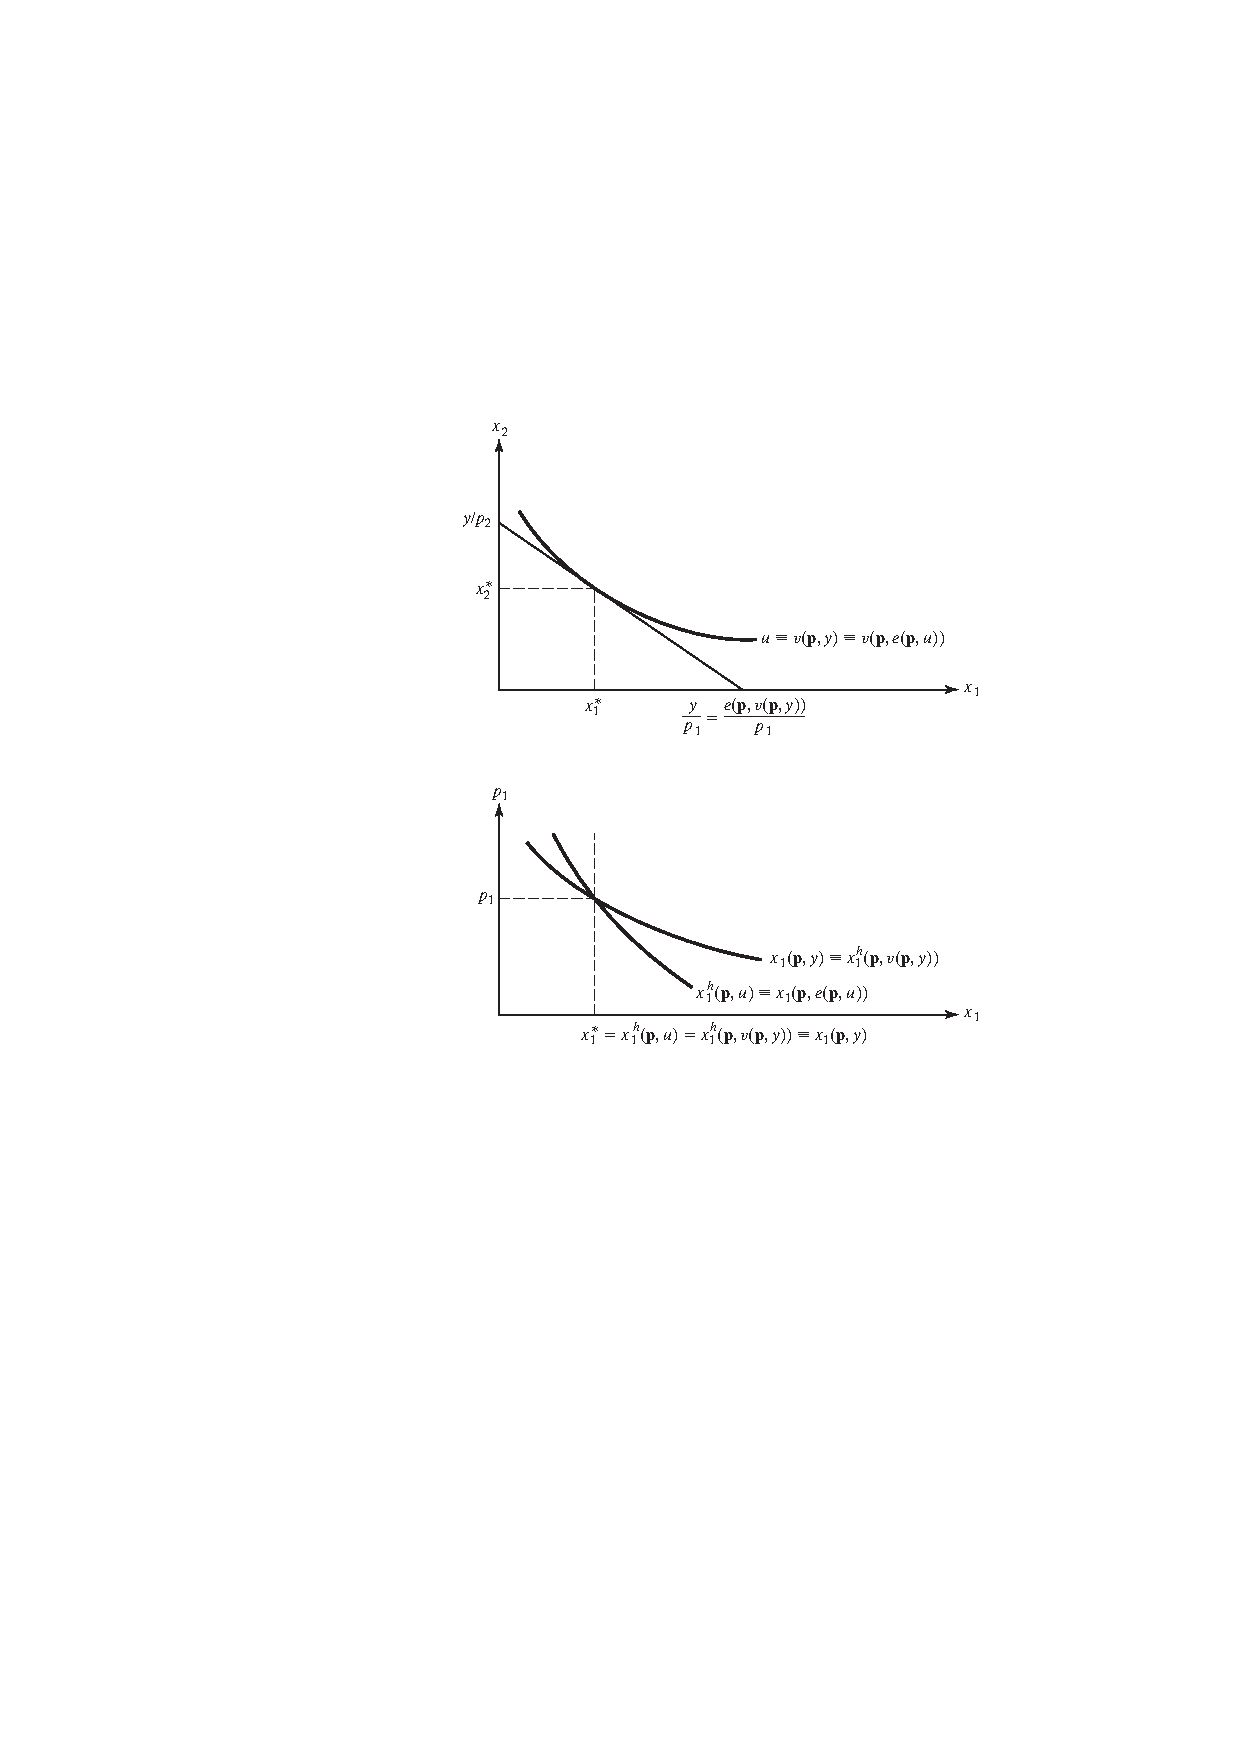
\includegraphics[width=10cm]{fig13.pdf}
  \caption{定理\ref{thm:thm1.3}和\ref{thm:thm1.4}的图示.}\label{fig1.13}
\end{figure}
\newpage
\section{消费者的性质}
\subsection{收入效应与替代效应}
在消费者行为模型中, 一个重要的问题是当价格变动时需求数量如何变动. 一般地, 我们倾向于认为在其他条件不变时, 若某商品价格下降, 消费者会多买一些, 若价格上升, 她会少买一些, 然而图\ref{fig1.14}表明实际情况并非如此.

在图\ref{fig1.14}中, 总是假设消费者是追求效用最大化的, 她的偏好是严格单调和凸的, 且她面对的价格是市场决定的. 在第1张图中, 商品1价格下降导致其需求量上升; 在第2张图中, 商品1价格下降但其需求量不变; 在第3张图中, 商品1价格下降导致其需求量绝对减少.
\begin{figure}[htbp!]
  \centering
  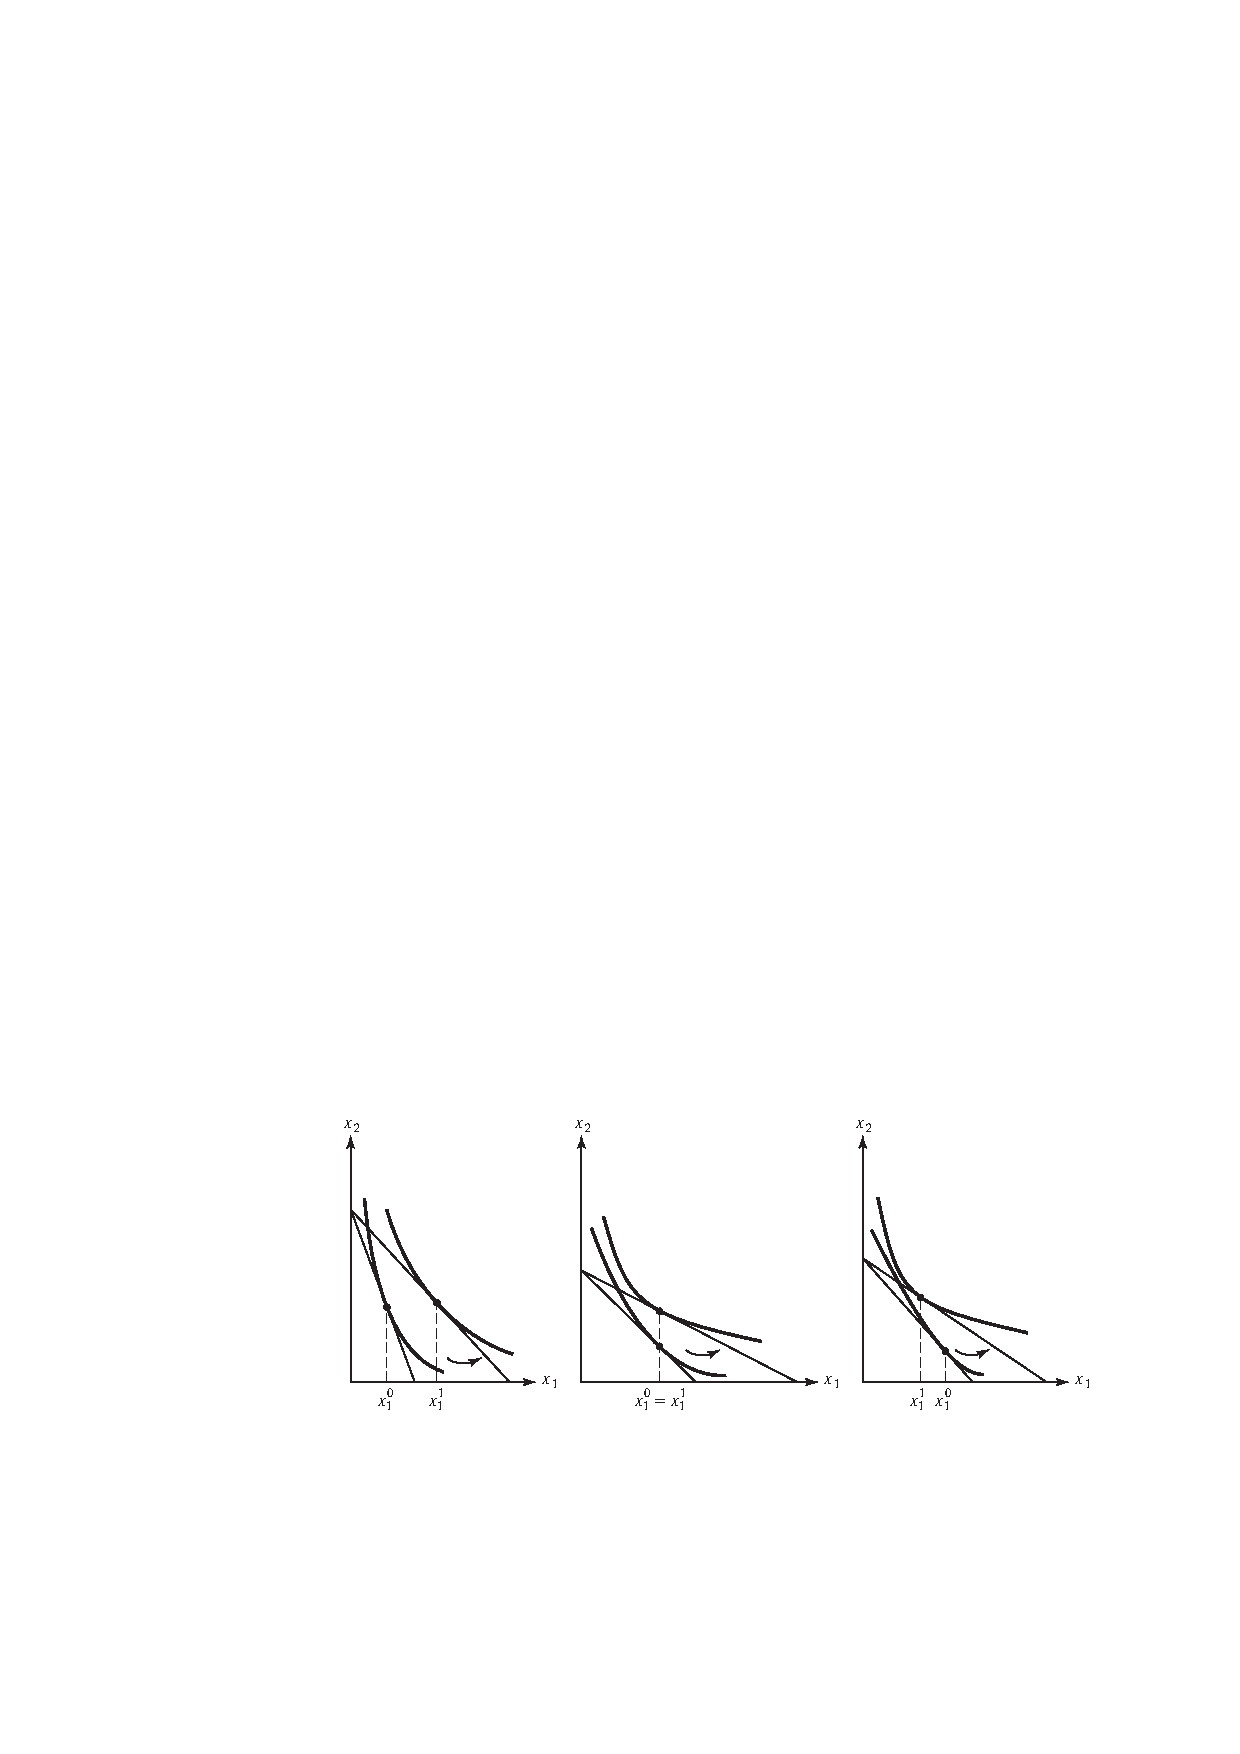
\includegraphics[width=15cm]{fig14.pdf}
  \caption{需求量对价格变动的反应.}\label{fig1.14}
\end{figure}

一方面, 商品1与其他商品相比该商品变得相对便宜了. 由于消费者想要所有各种商品, 即使消费者对所有商品的总购买力不变, 我们也可以预期他会用相对便宜的商品替代现在变得更昂贵的商品. 这种由于相对价格变动对需求量产生的效应称为\textbf{替代效应} (Substitution Effect, SE).

另一方面, 当某商品价格下降时, 消费者对所有商品的购买力实际上增加了, 这使得他会改变消费束中的某些或全部种类商品的数量, 只要他愿意. 这种由于购买力变动而对需求量产生的效应称为\textbf{收入效应} (Income Effect, IE).

价格变动的\textbf{总效应} (Total Effect, TE)为替代效应和收入效应之和, 这种分解可以遵循Hicks的方法来进行.

如图\ref{fig1.15}所示, 消费者最初面对的价格为$p_1^0$和$p_2^0$, 她的收入水平为$y$, 最初的购买量为$x_1^0$和$x_2^0$, 并且可以达到效用水平$u^0$. 现在假设商品1的价格从$p_1^0$下降到$p_1^1$而商品2的价格$p_2^0$维持不变, 价格变动的总效应体现为商品1的消费量增加至$x_1^1$而商品2的消费量下降至$x_2^1$.

现在对TE进行Hicks分解, 假想允许商品1的价格下降到$p_1^1$但维持效用水平$u^0$不变, 这种情形仿佛是允许消费者面对新的相对价格, 但却减少她的收入使得假想的预算约束线 (以虚线表示)与原本的平行, 此时消费者会增加商品1的消费量至$x_1^s$而将商品2的消费量减少至$x_2^s$, 这种价格变动就是商品1和商品2的Hicks替代效应. 现在只需解释消费量从$x_1^s$至$x_1^1$以及从$x_2^s$至$x_2^1$的变化, 这恰好是在新的价格水平和原有效用水平$u^0$时, 增加消费者的实际收入使得假想预算线平移至最终的预算线, 使得它与无差异曲线$u^1$相切, 这种价格变动称为商品1和商品2的Hicks收入效应, 描述的是纯粹由收入变动引起的需求量变动.

另一方面, 图\ref{fig1.15}显示了点$(p_1^0,x_1^0)$和$(p_1^1,x_1^1)$都在商品1的Marshall需求曲线上, 而点$(p_1^0,x_1^0)$和$(p_1^1,x_1^s)$都是商品1的Hicks需求曲线上. 换言之, Marshall需求曲线描述的是自价格 (own-price)变动引起的总效应, Hicks需求曲线描述的是自价格变动引起的纯Hicks替代效应, 两者差别可由Hicks收入效应解释.
\begin{figure}
  \centering
  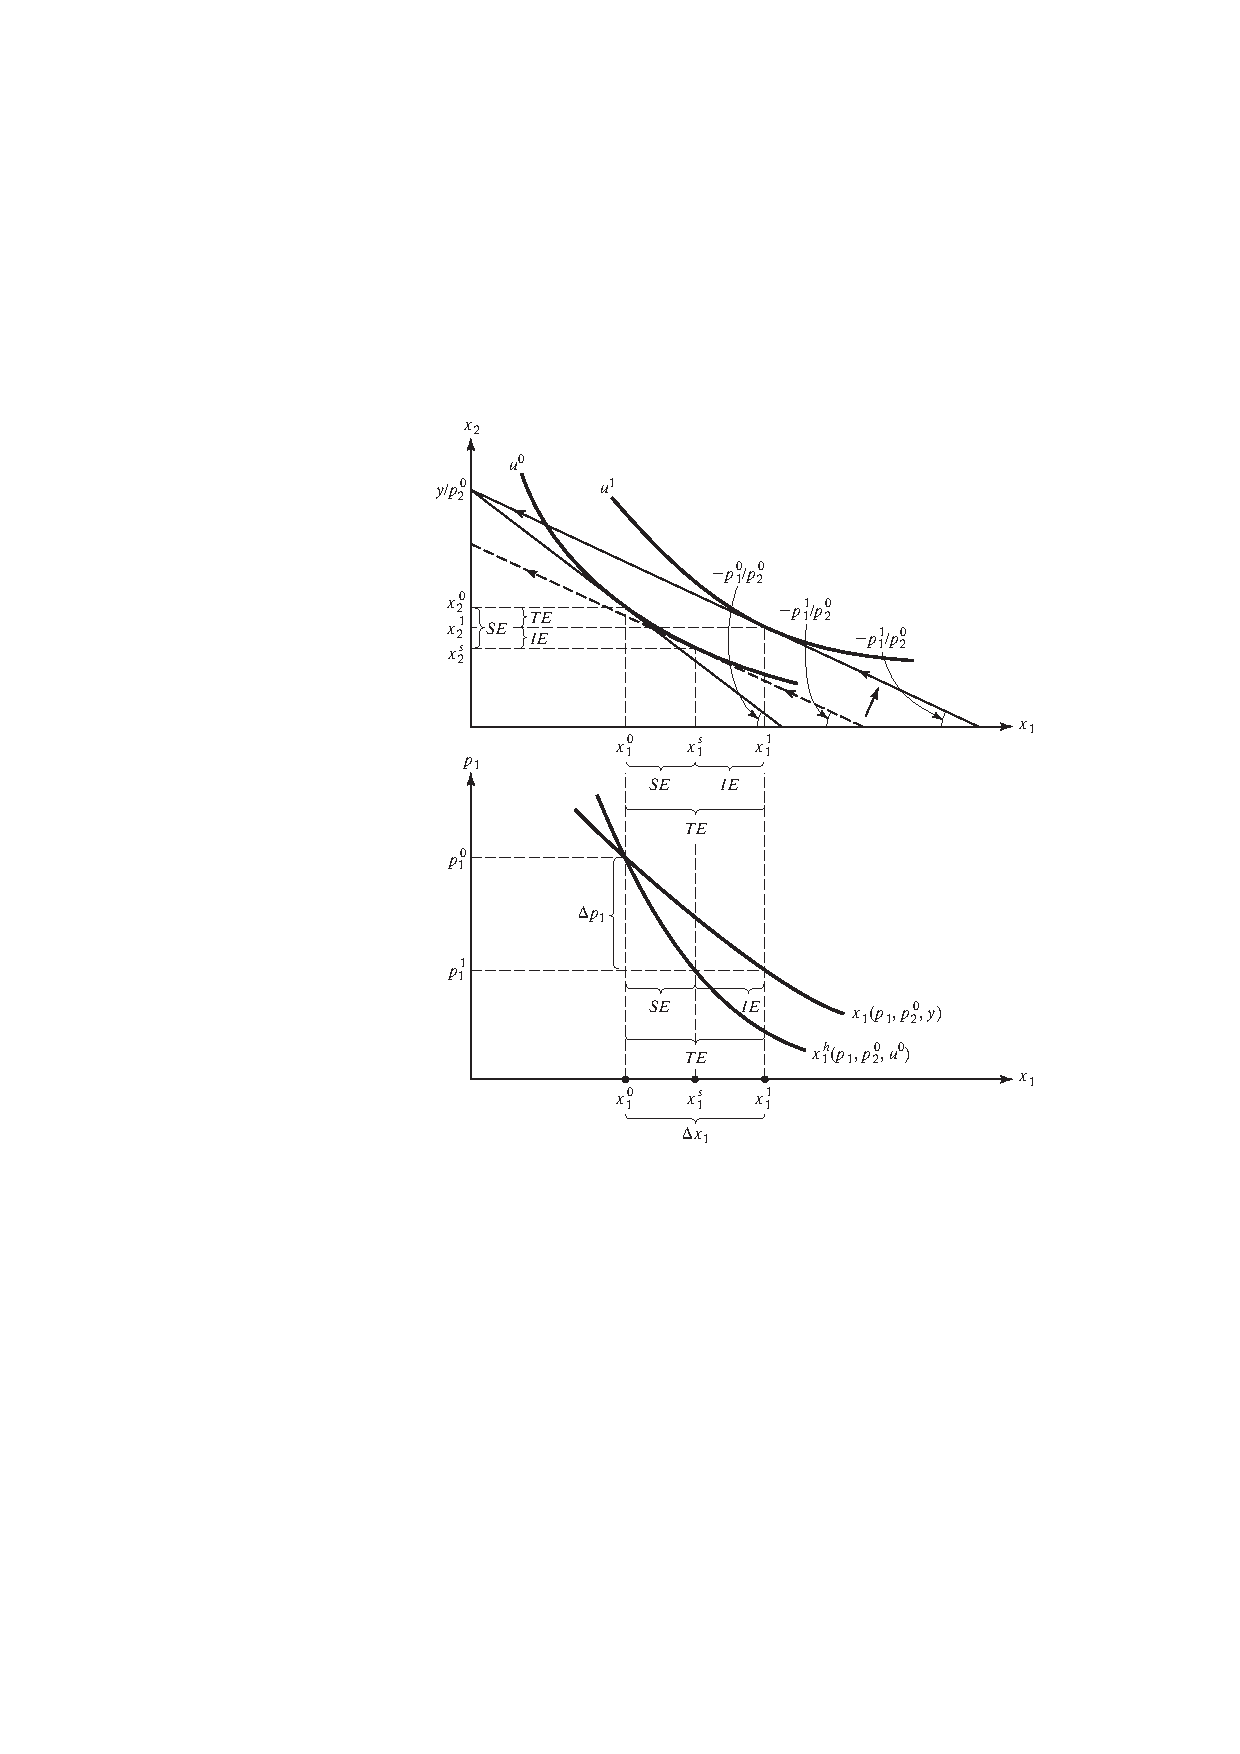
\includegraphics[width=10cm]{fig15.pdf}
  \caption{价格变动的Hicks分解.}\label{fig1.15}
\end{figure}

更一般地, 总效应、替代效应和收入效应可以用Slutsky方程表示, 它又称为“需求理论的基本方程”. 在接下来的部分, 总是规定假设\ref{pos:pos1.2}成立, 并且在需要时可以对函数微分.

\begin{theorem}[Slutsky方程]
  设$\x(\p,y)$表示消费者的Marshall需求方程组, 那么对于一切$(\p,y)\in\R_{++}^n\times\R_+$和$u=v(\p,y)$都有
  $$\frac{\partial x_i(\p,y)}{\partial p_j}=\frac{\partial x_i^h(\p,u)}{\partial p_j}-x_j(\p,y)\frac{\partial x_i(\p,y)}{\partial y},\quad i,j=1,\cdots,n$$
\end{theorem}
\begin{proof}
  根据定理\ref{thm:thm1.4}可知
  $$x_i^h(\p,u)=x_i(\p,e(\p,u))$$
  对于任意$\p\gg\mathbf{0}$和效用水平$u$成立, 上式两端同时对$p_j$微分得
  \begin{equation}\label{eq1.22}
    \frac{\partial x_i^h(\p,u)}{\partial p_j}=\frac{\partial x_i(\p,e(\p,u))}{\partial p_j}+\frac{\partial x_i(\p,e(\p,u))}{\partial y}\frac{\partial e(\p,u)}{\partial p_j}
  \end{equation}
  由于$u=v(\p,y)$是价格为$\p$收入为$y$时消费者所能实现的最大效用水平, 根据定理\ref{thm:thm1.3}可得
  \begin{equation}\label{eq1.23}
    e(\p,u)=e(\p,v(\p,y))=y
  \end{equation}
  根据Shephard引理可知
  $$\frac{\partial e(\p,u)}{\partial p_j}=x_j^h(\p,u)=x_j^h(\p,v(\p,y))$$
  再根据定理\ref{thm:thm1.4}可知
  \begin{equation}\label{eq1.24}
    \frac{\partial e(\p,u)}{\partial p_j}=x_j(\p,y)
  \end{equation}
  将式(\ref{eq1.23})和(\ref{eq1.24})代入到(\ref{eq1.22}), 稍加整理即可得到
  $$\frac{\partial x_i(\p,y)}{\partial p_j}=\frac{\partial x_i^h(\p,u)}{\partial p_j}-x_j(\p,y)\frac{\partial x_i(\p,y)}{\partial y}$$
  结论成立.
\end{proof}

Slutsky方程告诉我们总效应可以被分解为可观测到的收入效应和不可观测的替代效应, 根据该方程, 为了解释Marshall需求曲线的斜率 (需求量对自价格变动的反应), 必须知道Hicks需求曲线, 然而它是不可观测的, 但仍可以从消费者理论中获取它的信息.

\begin{theorem}
  设$x_i^h(\p,u)$是商品$i$的Hicks需求曲线, 那么$\partial x_i^h(\p,u)/\partial p_i\le0$.
\end{theorem}
\begin{proof}
  根据Shephard引理可知对任意$(\p,u)\in\R_{++}^n\times\mathcal{U}$都有
  $$\frac{\partial e(\p,u)}{\partial p_i}=x_i^h(\p,u)$$
  两边再对$p_i$求微分得
  $$\frac{\partial^2e(\p,u)}{\partial p_i^2}=\frac{\partial x_i^h(\p,u)}{\partial p_i},\quad i,j=1,\cdots,n$$
  由于$e$是关于$\p$的凹函数, 因此二阶偏导数非正, 由此证得命题.
\end{proof}
这一定理表明任何商品$i$的替代效应均非正, 因此当商品$i$的价格下降时, 替代效应必然非负, 但正如图\ref{fig1.14}所描述的那样, 商品价格下降时, 总效应也可能非正, 也即它的消费量也会下降, 称为Giffin悖论. 如果一种商品的需求量随着收入上升而增加, 则称它为\textbf{正常品} (normal good), 如果它的需求量随着收入上升而下降, 则称它为\textbf{劣等品} (inferior good).

\begin{corollary}
正常品的自价格下降会导致它的需求量上升; 如果商品自价格下降导致它的需求量减少, 那么该商品必定为劣等品.
\end{corollary}

为了了解更多关于替代效应的信息, 有必要继续探讨替代项的性质, 首先证明“交叉-替代项”是对称的.

\begin{proposition}\label{pro:pro1.3}
设$\x^h(\p,u)$表示消费者的Hicks需求方程组, 并且$e$是二阶连续可微的, 那么
$$\frac{\partial x_i^h(\p,u)}{\partial p_j}=\frac{\partial x_j^h(\p,u)}{\partial p_i},\quad i,j=1,\cdots,n$$
\end{proposition}
\begin{proof}
  根据Shephard引理可知
  $$\frac{\partial}{\partial p_j}\left[\frac{\partial e(\p,u)}{\partial p_i}\right]=\frac{\partial x_i^h(\p,u)}{\partial p_j}$$
  它等价于
  \begin{equation}\label{eq1.25}
    \frac{\partial^2e(\p,u)}{\partial p_j\partial p_i}=\frac{\partial x_i^h(\p,u)}{\partial p_j}
  \end{equation}
  对于一切$i,j=1,\cdots,n$成立, 根据Young定理可知, 支出函数的交叉二阶偏导的顺序是无所谓的, 也即
  $$\frac{\partial^2e(\p,u)}{\partial p_j\partial p_i}=\frac{\partial^2e(\p,u)}{\partial p_i\partial p_j}$$
  将该式与式(\ref{eq1.25})联立即可证得命题.
\end{proof}

\begin{proposition}\label{pro:pro1.4}
设$\x^h(\p,u)$表示消费者的Hicks需求, 并且
$$\sigma(\p,u)=\begin{pmatrix}
                 \frac{\partial x_1^h(\p,u)}{\partial p_1} & \cdots & \frac{\partial x_1^h(\p,u)}{\partial p_n} \\
                 \vdots &  & \vdots \\
                 \frac{\partial x_n^h(\p,u)}{\partial p_1} & \cdots & \frac{\partial x_n^h(\p,u)}{\partial p_n}
               \end{pmatrix}$$
为包含所有Hicks替代项的替代矩阵, 那么$\sigma(\p,u)$是半负定的.
\end{proposition}
\begin{proof}
  根据式(\ref{eq1.25})可得
  $$\begin{pmatrix}
                 \frac{\partial x_1^h(\p,u)}{\partial p_1} & \cdots & \frac{\partial x_1^h(\p,u)}{\partial p_n} \\
                 \vdots &  & \vdots \\
                 \frac{\partial x_n^h(\p,u)}{\partial p_1} & \cdots & \frac{\partial x_n^h(\p,u)}{\partial p_n}
               \end{pmatrix}=\begin{pmatrix}
                               \frac{\partial^2 e(\p,u)}{\partial p_1^2} & \cdots & \frac{\partial e(\p,u)}{\partial p_n\partial p_1} \\
                               \vdots &  & \vdots \\
                               \frac{\partial^2 e(\p,u)}{\partial p_1\partial p_n} & \cdots & \frac{\partial^2 e(\p,u)}{\partial p_n^2}
                             \end{pmatrix}$$
  上式右端的矩阵是支出函数$e$关于价格$\p$的Hessian矩阵, 由于$e$是$\p$的凹函数, 故而该矩阵为半负定的.
\end{proof}
\begin{theorem}\label{thm:thm1.5}
  设$\x(\p,y)$是消费者的Marshall需求方程组, 定义第$(i,j)$个Slutsky项为
  $$s_{ij}=\frac{x_i^h(\p,u)}{\partial p_j}+x_j(\p,y)\frac{\partial x_i(\p,y)}{\partial y}$$
  那么Slutsky矩阵$s(\p,y)=(s_{ij})_{n\times n}$是对称和半负定的.
\end{theorem}
\begin{proof}
  设$u$是价格为$\p$收入为$y$时, 消费者效用可以达到的最大值, 于是$u=v(\p,y)$. 根据Slutsky方程可得第$(i,j)$个替代项为
  $$\frac{x_i^h(\p,u)}{\partial p_j}=\frac{x_i(\p,y)}{\partial p_j}+x_j(\p,y)\frac{\partial x_i(\p,y)}{\partial y}$$
  于是Slutsky矩阵$s(\p,y)$的每一个元素恰好等于Hicks替代矩阵$\sigma(\p,u)$的相应元素. 根据命题\ref{pro:pro1.3}可知替代矩阵关于$u$是对称的, 而命题\ref{pro:pro1.4}又表明替代矩阵关于$u$是半负定的, 结论成立.
\end{proof}
定理\ref{thm:thm1.5}表明, 可以使用替代矩阵的知识推断出所有价格和收入变动对可观测的Marshall需求方程组的影响.
\subsection{弹性关系}
设$x_i(\p,y)$是消费者的Marshall需求函数, 预算平衡指的是对于每组价格和收入, 预算约束必然以等式形式成立, 也即
$$y=\sum_{i=1}^{n}p_ix_i(\p,y)$$
对一切$\p$和$y$成立, 因而如果任意单个商品价格或收入变动, 上式在变动前后仍成立. 因此, 消费者所有需求对价格和收入变动的反应需按照某种方式加总, 且这种方式要能保留变化发生后预算约束的等式仍然成立的这一性质, 为此需要介绍一些新的定义.

\begin{definition}
设$x_i(\p,y)$是消费者的Marshall需求函数, 那么
$$\eta_i=\frac{\partial x_i(\p,y)}{\partial y}\frac{y}{x_i(\p,y)}$$
称为商品$i$的收入弹性 (income elasticity), 并且
$$\epsilon_{ij}=\frac{\partial x_i(\p,y)}{\partial p_j}\frac{p_j}{x_i(\p,y)}$$
称为商品$i$的需求价格弹性 (demand price elasticity), 以及
$$s_i=\frac{p_ix_i(\p,y)}{y}$$
称为商品$i$的收入份额 (income share).
\end{definition}

$\eta_i$衡量的是消费者收入变动1\%导致商品$i$需求量变动的百分比. $\epsilon_{ij}$衡量的是价格$p_j$变动1\%引起的商品$i$需求量变动的百分比, 如果$j=i$, 则$\epsilon_{ij}$称为\textbf{自价格弹性} (own-price elasitcity), 如果$j\ne i$, 则$\epsilon_{ij}$称为关于$p_j$的\textbf{交叉价格弹性} (cross-price elasticity). $s_i$表示消费者花费在商品$i$上的金额占总收入的比例, 显然有$s_i\ge0$且$\sum_{i=1}^{n}s_i=y$.

\begin{theorem}
  设$\x(\p,y)$是消费者的Marshall需求方程组, 那么以下关系成立
  \begin{enumerate}[label=\arabic*.]
    \item Engle加总: $\sum_{i=1}^{n}s_i\eta_i=1$;
    \item Cournot加总: $\sum_{i=1}^{n}s_i\epsilon_{ij}=-s_{ij}$, $j=1,\cdots,n$.
  \end{enumerate}
\end{theorem}
\begin{proof}
  1. 首先预算约束要求
  \begin{equation}\label{eq1.26}
    y=\p\cdot\x(\p,y)
  \end{equation}
  对一切价格$\p$和收入$y$成立, 上式两端对$y$求导得
  $$1=\sum_{i=1}^{n}p_i\frac{\partial x_i}{\partial y}$$
  上式右端同时乘以和除以$x_iy$得
  $$1=\sum_{i=1}^{n}\frac{p_ix_i}{y}\frac{\partial x_i}{\partial y}\frac{y}{x_i}$$
  也即$1=\sum_{i=1}^{n}s_i\eta_i$.
  
  2. 在式(\ref{eq1.26})两端对$p_j$求导得
  $$0=\left(\sum_{i\ne j}p_i\frac{\partial x_i}{\partial p_j}\right)+x_j+p_j\frac{\partial x_i}{\partial p_j}$$
  合并同类项并整理得到
  $$-x_j=\sum_{i=1}^{n}p_i\frac{\partial x_i}{\partial x_j}$$
  它等价于
  $$-\frac{p_jx_j}{y}=\sum_{i=1}^{n}\frac{p_ix_i}{y}\frac{\partial x_i}{\partial p_i}\frac{p_j}{x_i}$$
  也即$-s_j=\sum_{i=1}^{n}s_i\epsilon_{ij}$, $j=1,\cdots,n$.
\end{proof}
以上定理表明, 如果以收入份额为权重, 那么收入弹性的加权和为1 (Engle加总), 而需求价格弹性的加权和必定呈现出某种特别方式 (Cournot加总).
\chapter{消费者理论\rom{2}}
\end{document} 